\label{ch:delayedheat}

\section{MOAA}

% PHYSOR - PRELIM
The Irradiation Experiment Neutronics Analysis group at the \gls*{INL} supports the \gls*{ATR} and the \gls*{TREAT} by performing neutronics analyses before the irradiation of experiments takes place.
% MAYBE - add more details to this ?
% Why is necessary to calculate the source term
The analyses provide the radioisotope source term of the experiments after irradiation.
% Can we cite previous work ?
The calculated source terms have multiple applications, which include radiation shielding, inventory and shipping purposes, demonstration of compliance with the safety limits, modeling of radioactive material dispersion, comparison to \gls*{PIE} results for validation, and experiment design and optimization, among others.

% Objectives
This section introduces the MCNP-ORIGEN Activation Automation (MOAA) tool and explains its workflow.
% why is MOAA necessary
The Irradiation Experiment Neutronics Analysis group developed MOAA to streamline the calculation of the experiment source terms.
% What is MOAA
MOAA is a Python package that couples MCNP \cite{mcnp} and ORIGEN \cite{scale} by writing MCNP tally cards, reading MCNP tallies, creating SCALE input files, executing SCALE, and standardizing the results post-processing.
Streamlining this procedure helps to reduce processing times and avoid potential human errors.

Although MOAA was originally developed to analyze the irradiation of experiments at ATR, it has grown to become a more general tool through further development.
Overall, MOAA is a tool that calculates radionuclide mass, activity, and heat in the regions of interest in a nuclear reactor.
% Other potential applications
% cite previous work and applications
Similar tools set a path for potential future applications for MOAA, including fuel burnup \cite{sterbentz_agr1_2018}, spent fuel repository design \cite{spent_fuel_2008}, transportation cask design \cite{transportation_2016}, shutdown dose calculation \cite{chen_rigorous_2002}, to mention just a few.
Additionally, earlier work utilized MOAA for delayed heating calculations \cite{fairhurst_decay_2022, fairhurst_demonstration_2022, fairhurst_database_2022}.
% See if there is any report that I could cite
% burnup of reactor with moving inventory \cite is there a report maybe?


\subsection{Calculation Workflow}

% Intro: single/multiple irradiations
MOAA performs material irradiation and decay calculations, which can be configured to include a single or multiple irradiation steps \cite{fairhurst_development_2022}.
While a single-step calculation uses constant power irradiation, multi-step calculations can handle several core configurations and piecewise constant power irradiation (i.e., different power levels at each time step).
Such capability allows for the modeling of evolution in material density, temperature, and geometry, as well as the control rod movement during the irradiation cycle.
% Predictor/Corrector
Additionally, the calculations can be configured to utilize the conventional predictor-corrector scheme, which is a two-step process that combines explicit and implicit calculations to achieve higher accuracy.

% General workflow - describe what each component does
% Figure \ref{fig:workflow_1} shows the calculation of the isotopic composition $m_l$ after irradiation case $l$.
% The subsequent irradiation case uses $m_l$ to update the MCNP material definitions.
\begin{figure}[htbp!]
  \begin{center}
    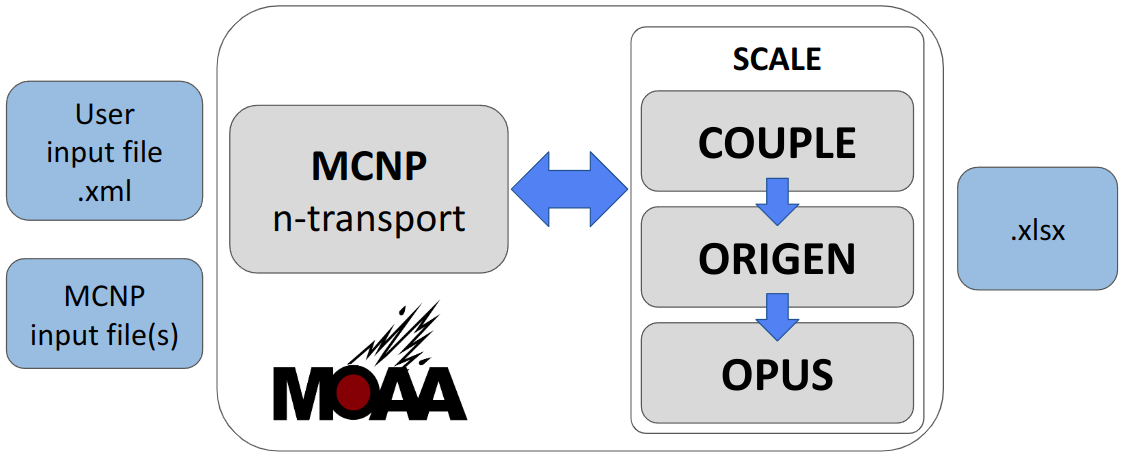
\includegraphics[scale=0.4]{figures/diagram_2}
  \end{center}
  \caption{Graphical representation of MOAA's workflow.}
  \label{fig:workflow_1}
\end{figure}

Figure \ref{fig:workflow_1} highlights MOAA's main calculation workflow that integrates with MCNP and ORIGEN.
MCNP is a general-purpose, continuous-energy, generalized-geometry, Monte Carlo radiation-transport tool that can track neutrons, photons, electrons, and other particles.
The main advantage of the Monte Carlo method is its capability to model geometry and interaction physics without significant approximations.
MOAA relies on MCNP for obtaining the geometry- and material-dependent parameters of the user-defined system during the irradiation steps - i.e., fluxes and reaction rates.

ORIGEN is a general-purpose point depletion and decay tool to calculate isotopic concentrations, radiation source terms, and decay heat.
ORIGEN is integrated into the SCALE code system, which is a modeling and simulation suite for nuclear safety analysis and design.
MOAA uses the calculated parameters from the MCNP output files to define the SCALE input files.
Besides ORIGEN, MOAA also uses the COUPLE and OPUS modules from SCALE.
ORIGEN requires a single volume- and spectrum-weighted cross-section library that MOAA generates using COUPLE.
Meanwhile, OPUS provides the ability to extract specific data from the ORIGEN output libraries, perform unit conversions, and generate data for post-calculation analysis.

% Formulas
MOAA calculates the following parameters for each cell of interest
% Need to double check the formulas
% isotopes: j
% reaction: k
% irradiation step: l
% predictor corrector: m = P or C
% irradiation case: l,m or n
\begin{align}
\phi(E)^{l, m} &= F4_{E} \\
\bar{\phi}_T^{l, m} &= \frac{\nu \times P [MW]}{Q [MeV/fiss] \times k_{eff} \times 1.6022 \times 10^{-19}} \times \mathlarger{\sum}_E F4_E \label{eq-flux} \\
\sigma_{j,k}^{l, m} &= \frac{ F4_{FM_{j,k}} }{ \mathlarger{\sum}_E F4_E } \\  % F4 tally_{FM}: the reaction cross-sections are microscropic (MCNP manual 3.3.5.7 Note 4)
k &= (n,\gamma), (n,p), (n,\alpha), (n,fission)
\end{align}
where $\phi(E)$ is the spectrum normalized to unity, $\bar{\phi}_T$ is the power-normalized total neutron flux, and $\sigma$ is the microscopic one-group cross-section.
The index $l$ corresponds to the irradiation step and index $m$ specifies the calculation to be the predictor or corrector case.
The index $j$ corresponds to the isotope identification number and index $k$ corresponds to the reaction type.
$F4_E$ is the F4 tally split up into energy bins, $F4_{FM_{j,k}}$ is the F4 tally for isotope $j$ reaction type $k$, $\nu$ is the number of neutrons emitted per fission, $P$ is the reactor power, $Q$ is the released energy per fission, and $k_{eff}$ is the effective multiplication factor.
MOAA extracts the parameters $\nu$, $k_{eff}$, $F4_E$, and $F4_{FM_{j,k}}$ from the MCNP output files, and $P$ and $Q$ are user-defined parameters.
A special use case is the ATR simulations in which $P$ has to be calculated.
Section \ref{sec:atr} gives further details on its calculation.

\begin{figure}[htbp!]
  \begin{center}
    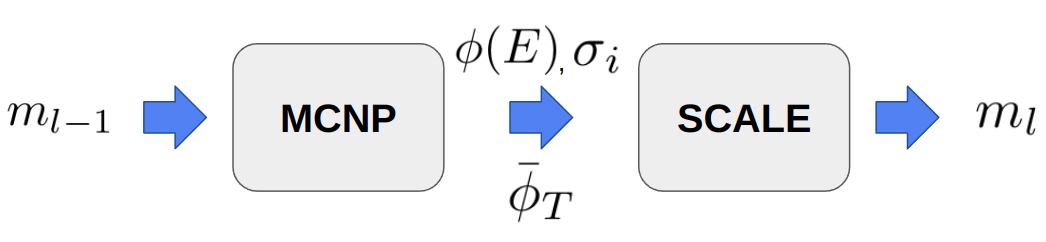
\includegraphics[scale=0.32]{figures/diagram_3}
  \end{center}
  \caption{Information flow of a MOAA simulation.}
  \label{fig:workflow_2}
\end{figure}

For multiple irradiation steps, MOAA calculates the isotopic composition at the end of the step $m_l$ based on the isotopic compositions from the previous step $m_{l-1}$, as shown in Figure \ref{fig:workflow_2}.
For the first irradiation step, the isotopic composition is extracted from the MCNP input file.
This method is known as constant extrapolation (CE) or Euler's method, which assumes that the flux and cross-sections remain at their beginning-of-step values throughout the interval \cite{leppanen_burnup_2012}.
If the predictor/corrector scheme is enabled, the irradiation step requires two irradiation calculations.
The first irradiation calculation uses $m_{l-1}$ to obtain $\phi(E)^{l, p}$, $\bar{\phi}_T^{l, p}$, and $\sigma_{j,k}^{p}$ to define the SCALE input files and calculate an intermediate isotopic composition $m_l^p$.
The second irradiation calculation uses $m_l^p$ to obtain $\phi(E)^{l, c}$, $\bar{\phi}_T^{l, c}$, and $\sigma_{j,k}^{c}$ and the following averaged parameters to define the SCALE input files and calculate $m_l$
% Predictor/Corrector formulas
\begin{align}
\phi(E) &= \frac{1}{2}\phi(E)^{l, p} + \frac{1}{2}\phi(E)^{l, c} \\
\bar{\phi}_T &= \frac{1}{2} \bar{\phi}_T^{l, p} + \frac{1}{2} \bar{\phi}_T^{l, c} \\
\sigma_{j,k} &= \frac{1}{2}\sigma_{j,k}^{l, p} + \frac{1}{2}\sigma_{j,k}^{l, c}.
\end{align}
This method is known as conventional predictor-corrector or constant extrapolation with linear interpolation (CE/LI) \cite{leppanen_burnup_2012}.
As the name suggests, the predictor calculation assumes constant values throughout the interval, and the final calculation uses an average of the predictor and corrector flux and cross-sections, which corresponds to a linear interpolation between the beginning and end-of-step values.

The creation of a MOAA application starts with the definition of a \gls*{UIF} in \textit{.xml} format, as shown in Figure \ref{fig:workflow_1}.
The UIF contains a set of required and optional settings for MOAA.
The required settings are a list of irradiation cases, a list of decay times, and a list of cells.
Within the irradiation cases, the user must specify an associated MCNP input file, an irradiation time, and an irradiation power.
% Basic user input description
Appendix \ref{ref:moaa-exec} displays a minimal MOAA input file.
MOAA's workflow can be summarized into Algorithm \ref{moaa_flow}.
If the predictor/corrector scheme is enabled, the number of cases is twice the number of irradiation cases.

\begin{algorithm}
  \caption{MOAA's main algorithm.}
  \label{moaa_flow}
  \begin{algorithmic}[1]
    \State parses user input file
    \For{case}
      \If {case $>$ 0}
        \State updates MCNP inputs with case-1 calculated compositions  
      \EndIf
      \State appends MCNP tallies
      \State executes MCNP
      \State parses MCNP output
      \If {case is corrector}
        \State applies correction
      \EndIf
      \State writes COUPLE sequence
      \State writes ORIGEN sequence
      \State writes OPUS sequence
      \State executes SCALE
      \State processes results
    \EndFor
  \end{algorithmic}
\end{algorithm}



\subsection{ATR cases}
\label{sec:atr}

The definition of an ATR case uses the same flux normalization as Equation \ref{eq-flux}, but requires the specification of the different lobe powers, as well as the calculation of adjusted lobe powers.
The adjusted lobe power can be thought of as a ``virtual'' total reactor power that would produce the same flux level in that lobe.
For experiments in lobes northwest (NW), northeast (NE), center (C), southwest (SW), and southeast (SE), the flux normalization uses the adjusted lobe power of the user-specified lobe powers.
The flux normalization of experiments in the rest of the lobes uses a weighted power average of the closest lobes.
For example, the east lobe (E) power is calculated as an average between the power of lobes NE, C, and SE.
The following formula calculates the adjusted lobe powers

% The tally number has to be user-specified with atr_lp_tally_id.
\begin{align}
T_i = \mathlarger{\sum}_c F7_{c} \times m_c \\
f_i = \frac{T_i}{ \mathlarger{\sum}_j T_j } \times \mathlarger{\sum}_j LP_j \\
P_i = \frac{LP_i}{f_i} \times \mathlarger{\sum}_j LP_j
\end{align}
where $F7_{c}$ is the fission energy tally, $m_c$ is the mass, and index $c$ represents the cells integrating the lobe.
$LP_i$ is the user-defined power for lobe $i$ and $P_i$ is the adjusted lobe power.
% ATR input file
The required settings within the irradiation cases include an MCNP input file, an irradiation time, an irradiation power divided into five lobe powers: NW, NE, C, SW, SE.
Additionally, the user must provide the F7 tally identification number that will be used for adjusting the lobe powers.
Appendix \ref{ref:moaa-exec} displays a typical UIF for an ATR irradiation experiment.


\subsection{Quality Assurance and Version Control}
\label{sec:quality}

% Quality Assurance
Nuclear regulators require the implementation of a quality assurance program for all systems that prevent or mitigate the consequences of postulated accidents in nuclear power plants and reprocessing plants.
Software plays a major role in licensing by producing calculations critical to the design and safety \cite{sqa}.
The implementation of a software quality assurance program ensures code reliability.

% NQA
This section briefly describes the current efforts for MOAA to fulfill the American Society of Mechanical Engineers (ASME) Nuclear Quality Assurance 1 (NQA-1) Standard \cite{nqa1}.
According to the NQA-1 documentation, ``this Standard reflects the current understanding of the quality assurance requirements necessary to achieve safe, reliable, and efficient utilization of nuclear energy, and management and processing of radioactive materials."
These requirements target different steps of the software development process, including \textit{software design requirements, software design, software implementation,} and \textit{software design verification}.
These steps entail the documentation of the entire process -- from the establishment of the software requirements to the confirmation that the design correctly fulfills them.
% 
The collection of these assets holistically qualifies MOAA for performing nuclear reactor physics analysis.
While this documentation discusses actions pertaining to the development of MOAA, MCNP and SCALE respective requirements are beyond the scope of this work.

% Releases
The NQA-1 standard requires reviews and approvals for each stable release, and a software test plan details the verification process that leads to such a release.
% Verification / Testing
The verification process comprises design reviews, alternative calculations, and/or testing.
Testing is the process of comparing the behavior of the observed code against its expected behavior.
The type of output for the different tests may range from numerical verification to error handling testing, covering behavior from the common to the extreme.
MOAA uses ``dynamic" testing, including white and black box techniques, to attempt to identify defects by executing the software.
All tests have the same objective, which is to ensure that the system produces the expected output when executed with the prescribed input.
This mechanism helps to provide confidence that the software performs as intended \cite{testing}.

% Directory tree
\begin{figure}[htbp!]
  \begin{center}
    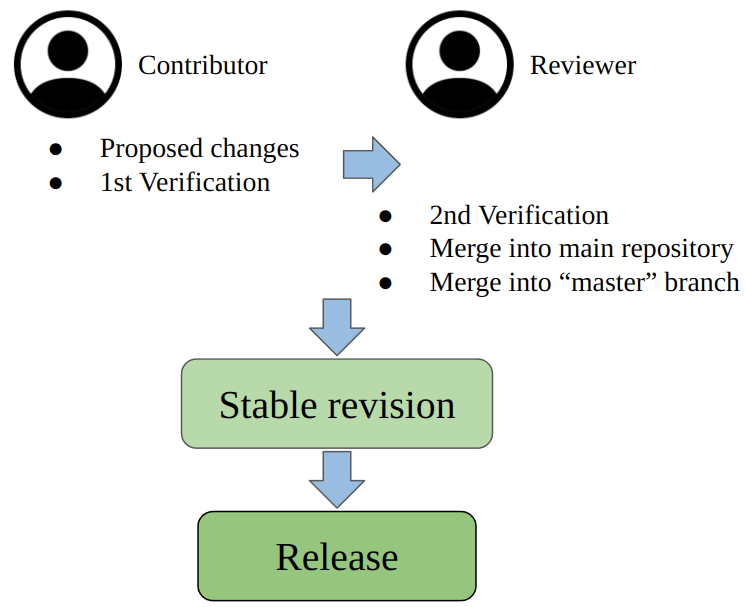
\includegraphics[scale=0.30]{figures/version-control}
  \end{center}
  \caption{Quality assurance process for MOAA.}
  \label{fig:sqa}
\end{figure}

% GitLab - Version Control
MOAA leverages the AGILE methodology for software development and tests that all proposed changes are properly integrated before merging them into the main repository hosting the source code, as shown in Figure \ref{fig:sqa}.
The proposed changes may include new features, which require the addition of new software design requirements, or a bug fix, which means that a software design requirement is not currently met.
After testing has been successfully completed (independently) by the contributor and a reviewer, a merge is made into the ``master" branch of the repository, creating a new ``stable" revision.
Each revision is eligible for release and subject to a complete release review.
Currently, a stable release of MOAA is under review.


\subsection{Simulation Specification}

To accommodate the MOAA calculations, the MCNP input files must undergo a few minimal modifications.
First, the depleted cells sharing the same material definition require the duplication of the original material, as each MOAA depleted cell requires an independent material definition.
The reason for this is to accommodate the depletion of independent cells subject to individual flux levels, divergent depletion rates, and the resulting different material compositions.

Second, while MOAA can handle the depletion of cells defined as repeated structures, it cannot handle the depletion when the same cell is present in different nested structures.
For example, if cell 100 is nested in cells 300 and 900 (100 $<$ 300 $<$ 900), and cell 100 is also nested in cells 400 and 900 (100 $<$ 400 $<$ 900), MOAA can handle only one of the two nested structures in one given simulation.
To handle both nested structures, cell 400 would have to be redefined as 300 if the geometry definition allows, and MOAA will be able to handle both occurrences simultaneously.

Third, the volume of some depleted cells has to be calculated and specified within the MCNP input file.
This is because MCNP can only calculate the volume of simple geometries only, and the user must specify the cell volumes to avoid errors.
For cells defined as repeated structures, the user must specify the volume of the whole material in those cells that is present in the geometry.
Otherwise, MCNP will calculate the volume of only one cell.


% Results
% Depletion results: AGR1 benchmark
\section{Delayed heating}

% This is probably repeated somewhere
In an operating reactor, an equilibrium exists between the generation and removal of heat.
After reactor shutdown, radioactive decay continues to release energy, which is deposited across the reactor and causes the delayed heating.
The estimation of delayed heating in experiments and in the reactor structures is paramount in the safety analyses of research reactors, and its accurate determination generates a reliable heat source term for thermal-hydraulics calculations.
This in turn allows the determination of heat removal requirements and evaluation of temperature levels in the components of interest \cite{fairhurst_decay_2022, fairhurst_machine_2022, fairhurst_machine_2_2022}.
Additionally, detailed calculations help in the optimization process of the irradiation target designs \cite{peterson-droogh_current_2018}.

Overall, these calculations determine whether delayed heating presents a hazard for the components of interest, which could lead to the release of radioactive contaminants into the reactor coolant.
An important application example is in spent nuclear fuel where delayed heating calculations are crucial for the design of nuclear facilities, including spent fuel storage pools, spent fuel transportation systems, reprocessing plants, and final storage sites.

% Objectives of the paper
This section introduces a delayed heating calculation workflow based on MOAA, presents the motivation for the choice of the method, and showcases its capabilities by presenting two specific applications.

\subsection{Calculation Workflow}
\label{sec:delheat}

Figure \ref{fig:workflow_0} summarizes the calculation workflow, which relies on the formal 3-step method for the delayed heating calculation.
During reactor operation, the first two steps in the formal 3-step process are accomplished by coupling a transport and a depletion solver.
The delayed heating calculation workflow presented here relies on the \gls*{MOAA} tool \cite{fairhurst_development_2022} for carrying out the first two steps.
After reactor shutdown, the depletion solver calculates the energy distribution and emission probability of the photon sources.
The photon-transport calculation uses this information to evaluate the delayed gamma heating.

%% General workflow
\begin{figure}[htbp!]
  \begin{center}
    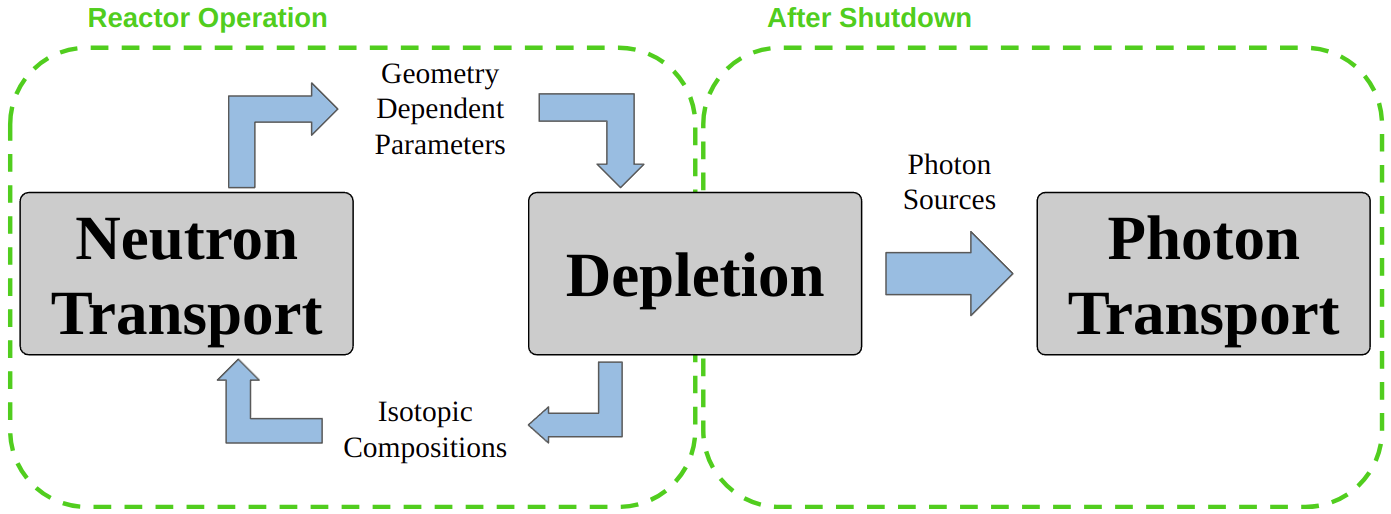
\includegraphics[width=0.80\linewidth]{figures/calc_w}
  \end{center}
  \caption{Calculation workflow diagram.}
  \label{fig:workflow_0}
\end{figure}

The delayed heating calculation can be separated into two parts.
The first part calculates the deposition of energy from charged particles $H_{ch}$.
This part includes only the charged particles that originated in the geometry of the component of interest and assumes that all the particles with mass deposit their energy in the region of interest.
The following equations calculate $H_{ch}$ \cite{giot_decay_2018, endf, peterson-droogh_current_2018}:

\begin{align}
H_{T, L} &= \mathlarger{\sum}_j N_j \lambda_j \bar{E}_j \\
H_{\gamma, L} &= \mathlarger{\sum}_j N_j \lambda_j \bar{E}_{EM, j} \\
\bar{E} &= \bar{E}_{EM} + \bar{E}_{HP} + \bar{E}_{LP} \\
\bar{E}_{EM} &= \bar{E}_{\gamma} + \bar{E}_{X-ray} + \bar{E}_{annih.rad.} + ... \\
\bar{E}_{HP} &= \bar{E}_{\alpha} + \bar{E}_{SF} + \bar{E}_{p} + ... \\
\bar{E}_{LP} &= \bar{E}_{\beta^-} + \bar{E}_{\beta^+} + \bar{E}_{Ae^-} + ... \\
H_{ch} [W] &= H_{T, L} - H_{\gamma, L}
\end{align}
where $H_{T, L}$ is the total decay heat, $N_j$ is the number of nuclei $j$, $\lambda_j$ is the decay constant of nucleus $j$, $\bar{E}_j$ is the total energy available (excluding neutrino energies) per decay of nucleus $j$, $H_{\gamma, L}$ is the total gamma heating, $\bar{E}_{EM}$ is the electromagnetic component, $\bar{E}_{HP}$ is the heavy particle component, $\bar{E}_{LP}$ is the light particle component, $\bar{E}_{\gamma}$ is the average gamma-ray energy, $\bar{E}_{x-ray}$ is the average X-ray energy, $\bar{E}_{annih.rad.}$ is the average annihilation energy, $\bar{E}_{\alpha}$ is the average $\alpha$ energy, $\bar{E}_{SF}$ is the average spontaneous fission energy, $\bar{E}_{p}$ is the average proton energy, $\bar{E}_{\beta^-}$ is the average $\beta^-$ energy, $\bar{E}_{\beta^+}$ is the average $\beta^+$ energy, and $\bar{E}_{Ae^-}$ is the average Auger-electron energy.

The second part calculates the deposition of energy from photons $H_{\gamma, Tr}$.
Because photons deposit their energy globally, photon transport is required, and this includes the photons originating from across the reactor.
The following equations describe the delayed heating
\begin{align}
H_{T} [W] &= H_{ch} + H_{\gamma, Tr}  \label{eq-heat} \\
H_{\gamma, Tr} [W] &= 1.6022 \times 10^{-13} \times \: ^* \! F8 [MeV] \times \mathlarger{\sum}_i S_i \label{eq-ga-tr} \\
S_i[\gamma/s] &= \int_{E} \varphi^\gamma_i(E) dE \\
s_i [-] &= S_i / \mathlarger{\sum}_j S_j \label{eq-emiprob}
\end{align}
where $H_{T}$ is the total heat deposited in the region of interest, $H_{ch}$ is the energy deposited in the region of interest by charged particles, $H_{\gamma, Tr}$ is the energy deposited in the region of interest resulting from the photon transport, $^\ast F8$ is the energy deposition calculated by an $^\ast$F8 tally, $S_i$ is the total photon emission rate from the region $i$, $\varphi^\gamma_i(E)$ the photon source energy distribution from region $i$, and $s_i$ is the source cell emission probability.

Overall, the calculation scheme follows the formal 3-step process, in which MOAA conducts the first two steps, and multiple MCNP photon-transport simulations conduct the third step, calculating the delayed gamma heating.
Figure \ref{fig:workflow_3} shows the calculation workflow.
MOAA calculates $H_{T,L}$ and $H_{\gamma, L}$ in the component of interest assuming those to be locally deposited.

\begin{figure}[htbp!]
  \begin{center}
    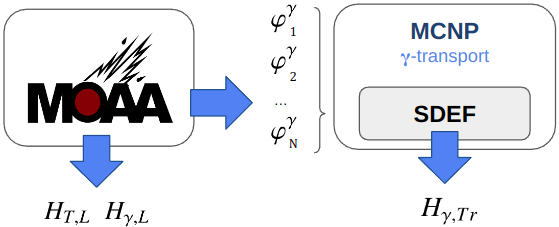
\includegraphics[width=0.70\linewidth]{figures/heat-flow}
  \end{center}
  \caption{Delayed heating calculation scheme relying on MOAA.}
  \label{fig:workflow_3}
\end{figure}

MOAA calculates $\varphi^\gamma_i(E)$ for all the cells defined by the user as contributors to the delayed heating.
The MCNP photon-transport simulations require the definition of a fixed source for these cells.
The source energy distribution is specified with $\varphi^\gamma_i(E)$.

The photon-transport calculation can be performed with multiple simulations, in which one simulation obtains the heat contribution for one source cell, or with one simulation, in which the simulation obtains the heat contribution for all the source cells simultaneously.
While the former determines the individual contributions from the different cells, the latter is computationally less expensive.
Nonetheless, the latter requires the definition of the cell emission probabilities $s_i$ using Equation \ref{eq-emiprob}.

The source spatial distribution is assumed uniform in each source cell.
For uniformly sampling the birth of a particle in a cell, MCNP uses the enclosing volume rejection method, which requires the user definition of a volume enveloping the source cell.
The randomly sampled points in the volume are accepted as source points only if they fall inside the source cell.
Finally, the photon transport estimates $^\ast F8$, which allows the calculation of $H_{\gamma, Tr}$ (Eq. \ref{eq-ga-tr}).


\subsection{Simulation Specification}

The calculation workflow requires the MOAA UIF and at least one MCNP input file defining the problem geometry.
However, the user may want to use different geometries for the neutron and photon transport and both MCNP input files should be defined.
This feature gives the calculation workflow great flexibility, allowing the user to model more complex scenarios.
For example, a study case can be the delayed heating sensitivity to long burnup in a reactor where there is fuel assembly shuffling.
Additionally, Chapter \ref{ch:sdr} studies cases where nuclear fuel is burned in the core, but the focus of the study is the shutdown dose rate for the \gls*{PIE}.

The delayed heating calculation requires two additional scripts: \texttt{run\_case.py} and \texttt{source\_gen.py}.
The script \texttt{run\_case.py} is the main workflow driver, and its role is summarized into Algorithm \ref{dh_flow}.

\begin{algorithm}
  \caption{Delayed heating main algorithm.}
  \label{dh_flow}
  \begin{algorithmic}[1]
    \State initializes delayed heating object
    \State reads source information
    \State creates neutron transport input files
    \State runs MOAA
    \State assigns lattice numbers to cells in repeated structures
    \State processes photon sources
    \State divides sources into batches
    \State creates photon transport input files
    \State runs MCNP for photon transport
    \State processes results
  \end{algorithmic}
\end{algorithm}

The script \texttt{source\_gen.py} allows for the automation of the photon source geometry definition.
This script defines the dimensions of the source where the particle birth is randomly sampled.
In the workflow described here, the user can define either a parallelepiped or a cylinder as the source geometry.
Appendix \ref{ap:mcnp_fixed} provides further details on the use of the delayed heating calculation workflow.


% Delayed Heating Results
\section{Results}
\label{sec:results}

This section presents and discusses the results of four exercises.
The first exercise is a code-to-code comparison between the workflow presented here and the Serpent Monte Carlo tool \cite{leppanen_serpent_2015}.
The second exercise demonstrates the calculation workflow for a simple case geometry.
The third exercise consists of the delayed heating calculation of an ATR experiment.
Finally, the fourth exercise analyzes the delayed heating in various structures in the RA-6 reactor.


\subsection{Delayed Gamma in a Uranium Sphere}

% Intro
This exercise studies the delayed gamma heating in a sphere of uranium.
The purpose of this study is to understand the foundation of the method by comparing the results with Serpent.
The Serpent Monte Carlo tool is a three-dimensional continuous-energy neutron transport application developed by the VTT Technical Research Centre of Finland, and it has been in public distribution since 2009.
This work uses Serpent 2.1.32 and the cross-section library ENDF/B-VII.0 for the calculations.
The choice of nuclear data was based on their availability.
This work uses Serpent because of its built-in burnup calculation routine.
Moreover, Serpent is capable of calculating delayed gamma heating in a two-step process.
The first step consists of a transport/depletion calculation that saves the radioactive material composition in a binary restart file.
The second step is a photon-transport simulation that generates the photon source based on the binary restart file.
This second simulation creates a \textit{\_gsrc.m} file specifying the gamma source distribution (see Appendix \ref{ap:serpent_gsrc} for further details).

The problem geometry includes a sphere of uranium surrounded by water, and it is shown in Figure \ref{fig:exp}.
The study focuses on the last component of equation \ref{eq-heat}, the heat generated by the transported gamma radiation $H_{\gamma, Tr}$.
% Describe model
The gamma heating is calculated after a 50 day-burnup at a constant power of 5 MW.

\begin{figure}[htbp!]
  \begin{center}
    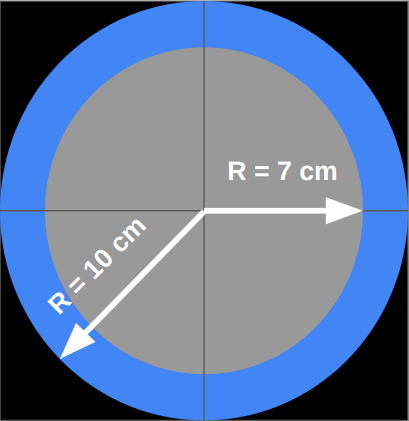
\includegraphics[width=0.35\textwidth]{figures/axial-view2}
  \end{center}
  \caption{Geometry of a sphere of uranium surrounded by water.}
  \label{fig:exp}
\end{figure}

% Results
The exercise compares the results of the nuclear heating calculation scheme developed here and Serpent.
Serpent provides the reference values for calculating the relative difference employing the following equation.
\begin{equation}
\textrm{Rel. Difference } [\%] = \frac{R_{\textrm{Serpent}} - R_{\textrm{MOAA}}}{R_{\textrm{Serpent}}} \times 100
\label{eq-rel-diff}
\end{equation}
where $R$ is the result of interest, which can be the integral flux, the mass of a nuclide, or gamma source intensity.

Table \ref{tab:gam-heat-results} summarizes the main results for different stages of the calculation.
The first stage is the burnup calculation.
The relative difference for the total neutron flux before burnup is below 1\%.
After burnup, the relative difference for the masses of U-235 and U-238 is below 1\% as well.

% Table
\begin{table}[htbp!]
  \centering
  \caption{Summary of the main results of the delayed heating calculation. $^1$ Before burnup. $^2$ After burnup.}
  \label{tab:gam-heat-results}
  \begin{tabular}{ccccc}
  % \begin{tabularx}{\textwidth}{ @{} L C{0.4} C{0.4} C{0.4} @{}}
    \toprule
                                & Units                     & MOAA/ MCNP & Serpent & Rel. Diff. [\%] \\
    \midrule
    $^1$Tot. neutron flux       & $10^{-3}/cm^{-2}/source$  & 3.9376  & 3.9284  & 0.24    \\
    $^2$U-235 mass              & $kg$                      & 25.279  & 25.279  & 0.01    \\
    $^2$U-238 mass              & $kg$                      & 2.835   & 2.835   & 0.01    \\
    $^2$Photon source intensity & $10^{17}\gamma/s$         & 10.16   & 4.65    & 118.40  \\
    $^2$Tot. gamma flux         & $10^{14}/cm^{-2}/s$       & 2.6464  & 1.7805  & 48.63   \\
    $^2$H$_{\gamma, Tr}$        & $kW$                      & 73.969  & 48.037  & 53.98   \\
    $^2$H$_{\gamma, Tr}/source$ & $10^{-14} \cdot J/source$ & 7.283   & 10.332  & -29.51  \\
    \bottomrule
  \end{tabular}
\end{table}

Figure \ref{fig:g-source} displays the gamma source distribution from radioactive decay after burnup.
MOAA uses 101 groups to obtain the source energy distribution and Serpent's data are formulated in the form of discrete lines.
There are some clear discrepancies around 10 keV between Serpent and MOAA caused by the Bremsstrahlung radiation.
While ORIGEN accounts for the photons originated by the deceleration of charged particles, Serpent considers only the photons originated directly from radioactive decays.
In opposition, the upper range of the source distribution shows better agreement.

MOAA predicts a photon source intensity more than two times greater than Serpent, as shown in Table \ref{tab:gam-heat-results}.
The origin of this discrepancy is mainly attributed to the consideration of the Bremsstrahlung radiation into the calculations.
Additionally, understanding the discrepancies requires some grasp of the algorithms in MOAA and Serpent.
In MOAA, COUPLE provides ORIGEN with the cross-section library necessary for the depletion calculation.
COUPLE creates by default spectrum-averaged cross-sections based on JEFF-3.0/A and replaces them with the cross-sections generated from the MCNP neutron transport calculation.
The cross-section values that are not replaced still use the JEFF spectrum-averaged cross-sections.
Monte Carlo solvers, such as MCNP and Serpent, track all necessary reaction rates and follow all the isotopes available in the nuclear data.
While MOAA relies primarily on ENDF/B-VII.1, it still depends on JEFF-3.0/A.
Consequently, MOAA and Serpent predict different after-burnup compositions, which translate into different photon source intensities.

\begin{figure}[htbp!] %or H 
    \centering
    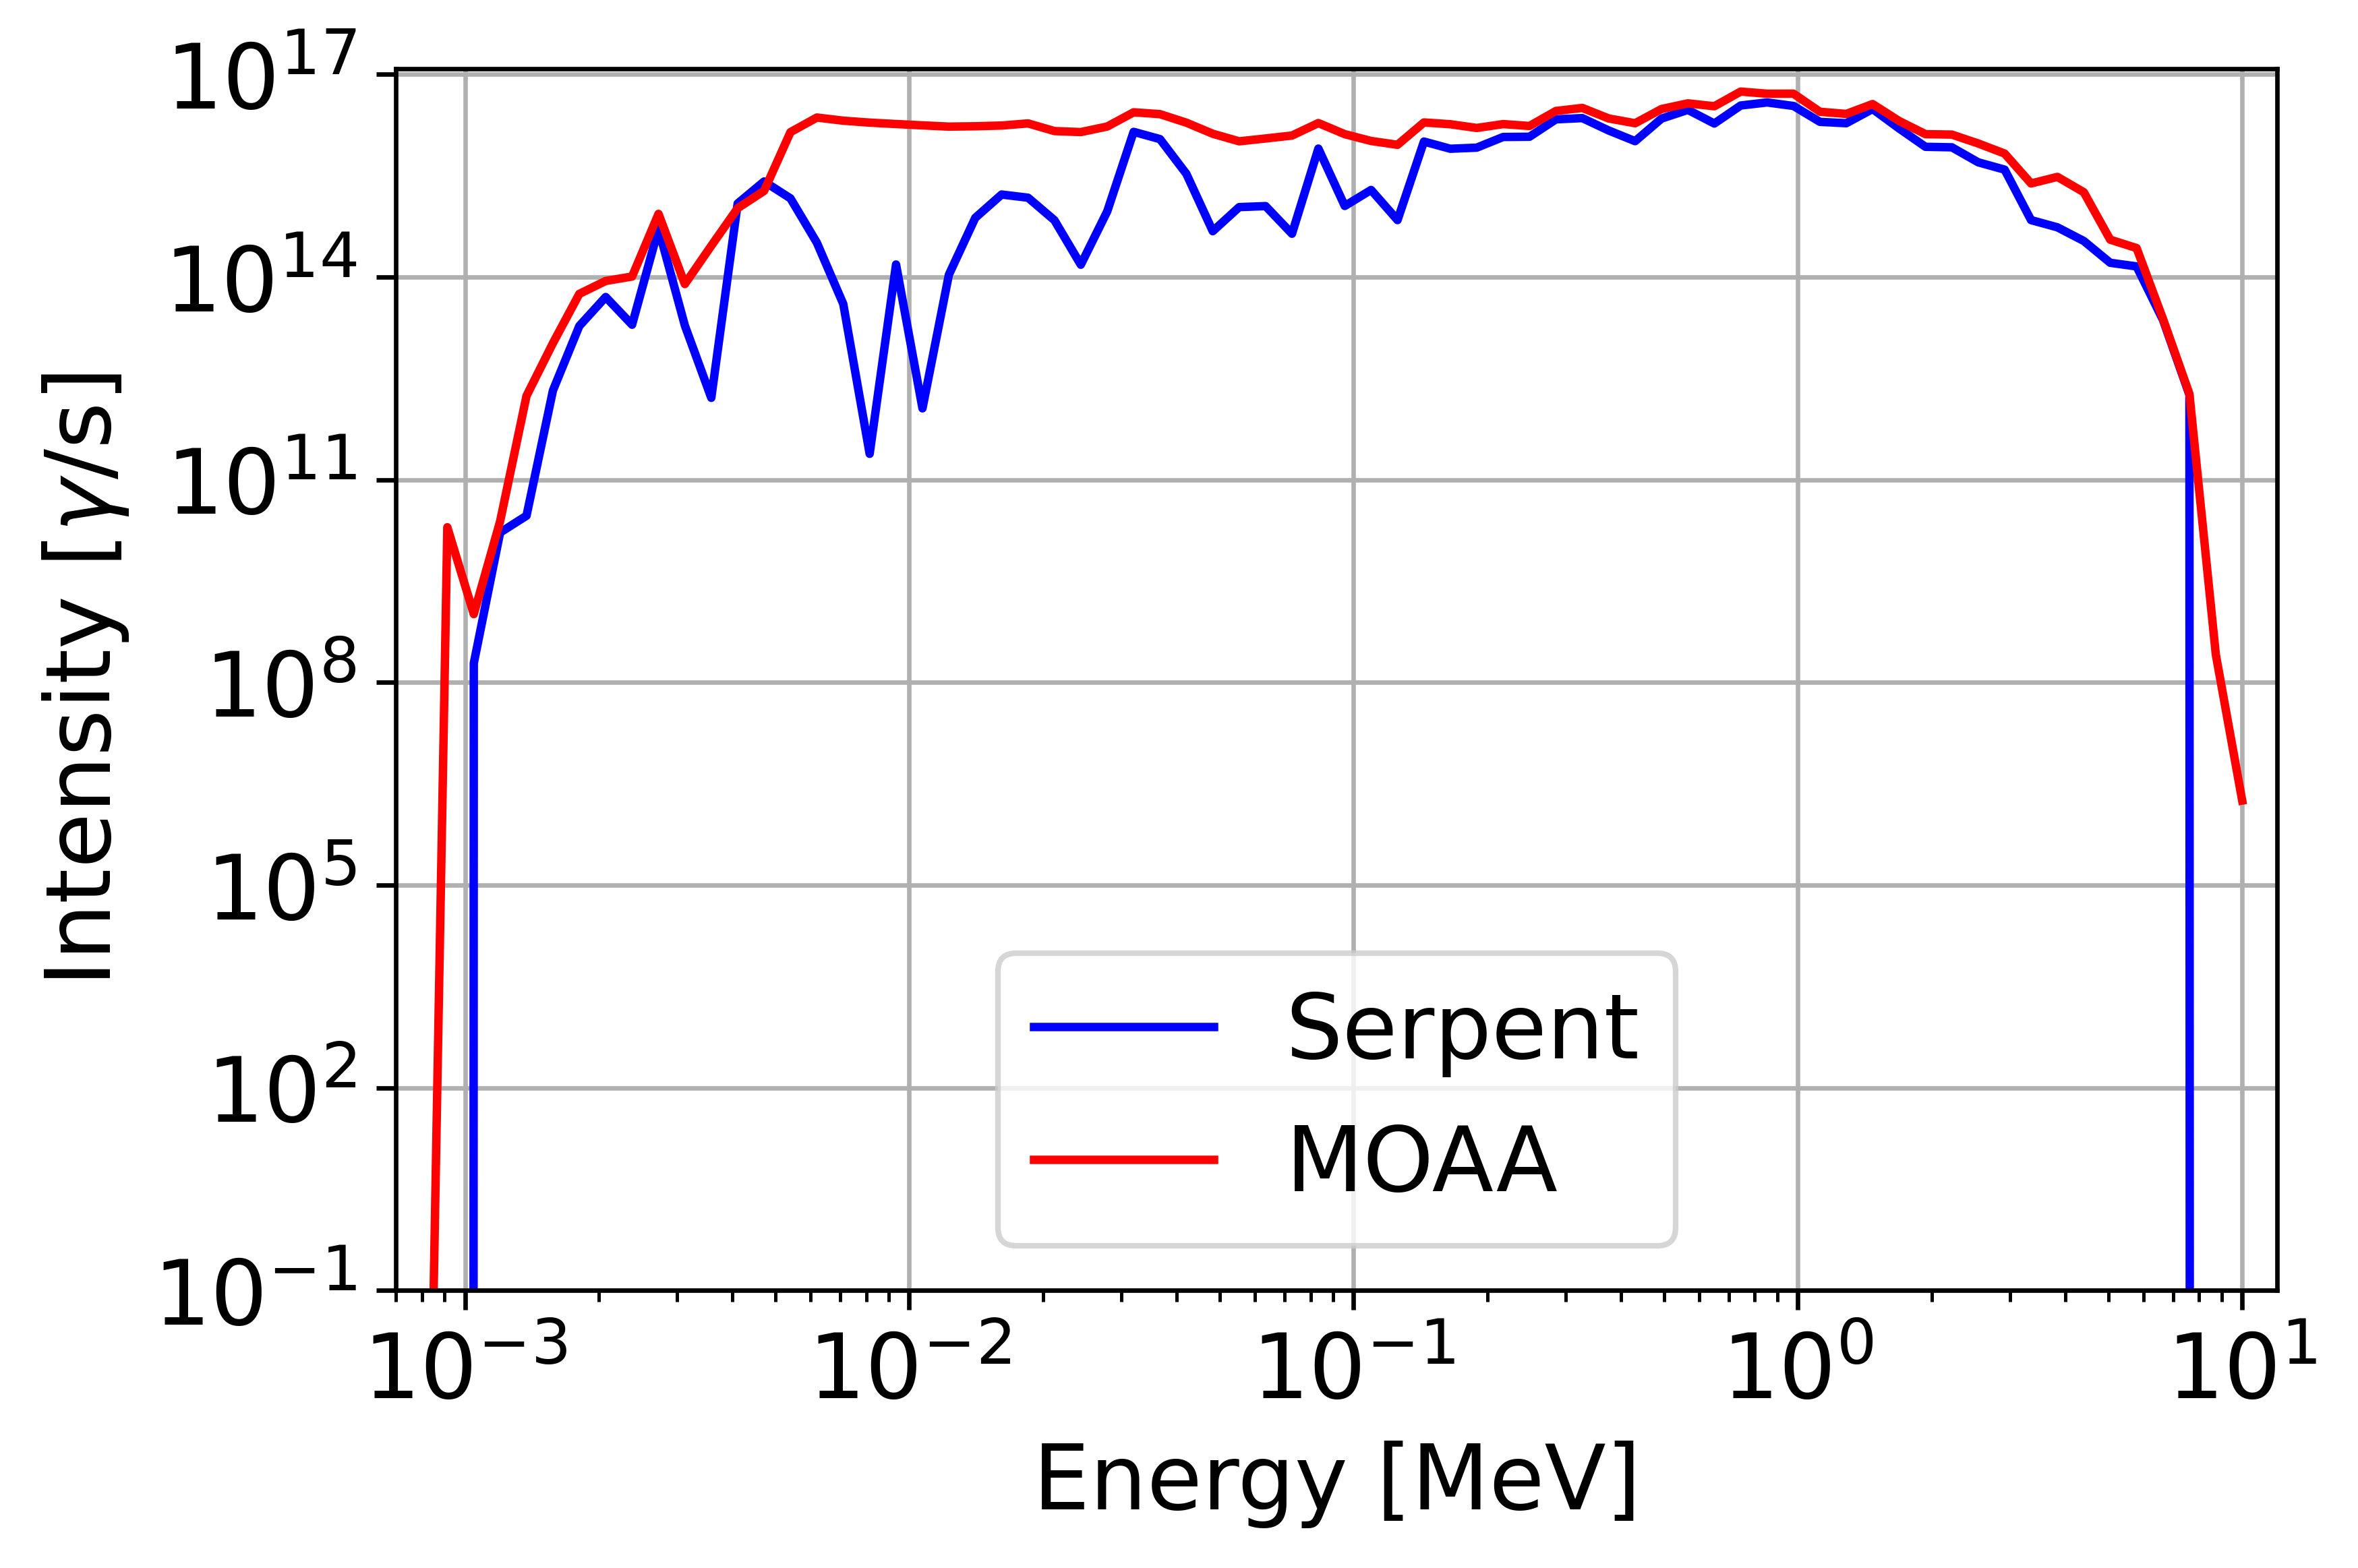
\includegraphics[width=0.6\linewidth]{figures/g-source.png}
    \hfill
    \caption{MOAA and Serpent photon source distributions.}
    \label{fig:g-source}
\end{figure}

Figure \ref{fig:g-spectra} displays the gamma spectra.
The largest discrepancy in the spectra is close to 10 keV.
MCNP fails to resolve some of the peaks in that area.
Additionally, the differences in gamma source distributions are carried over. 
Table \ref{tab:gam-heat-results} shows the results for the total gamma flux and the gamma heating.
Overall, the MCNP results are approximately 50\% larger than Serpent's.

Calculating the gamma heating per source particle, we can isolate the effects of the source intensity and source energy distribution on the results.
$H_{\gamma, Tr}/source$ in Table \ref{tab:gam-heat-results} shows the effects of the source energy distribution.
The MCNP value is 30\% smaller than Serpent's.
This last result confirms that the discrepancies in the total gamma flux and gamma heating are caused by the differences in both the source energy distribution and the source intensity.

% Gamma spectra
\begin{figure}[htbp!] %or H 
    \centering
    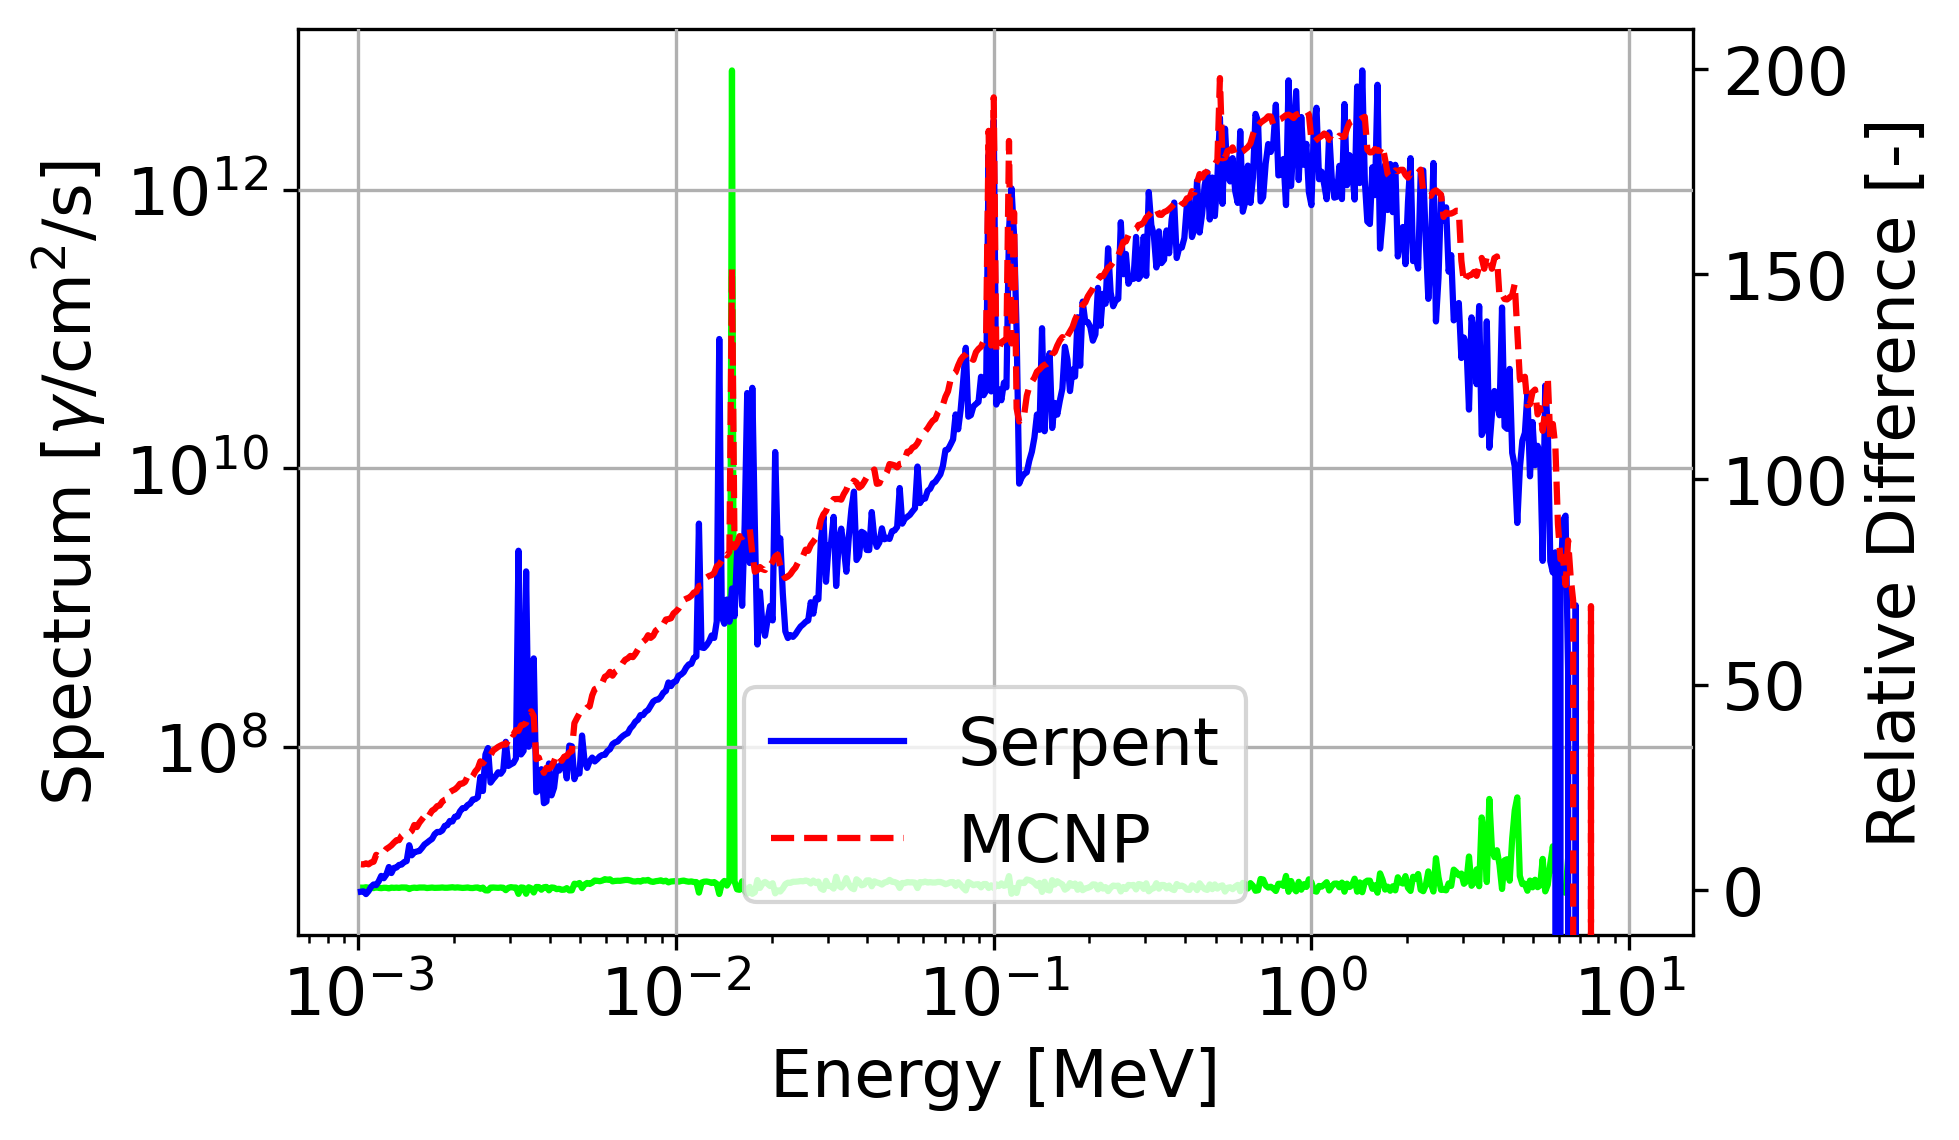
\includegraphics[width=0.65\linewidth]{figures/g-spect.png}
    \hfill
    \caption{MCNP and Serpent photon spectra.}
    \label{fig:g-spectra}
\end{figure}


\subsection{Demonstration Problem}
\label{sec:demo}
% From 14-

A top view of the exercise geometry and its dimensions are shown in Figure \ref{fig:toy-geo}.
The experiment center is located 8.2 cm away from the reactor center.
The fuel element and experiment heights are 14.8 and 24 cm, respectively.
The reactor encompasses the following materials: 85\% enriched uranium with a density of 19 g/cm$^3$ for the fuel elements, light water with a density of 1 g/cm$^3$ for the moderator, and iron with a density of 7.87 g/cm$^3$ for the experiment.

\begin{figure}[htbp!] %or H 
    \centering
    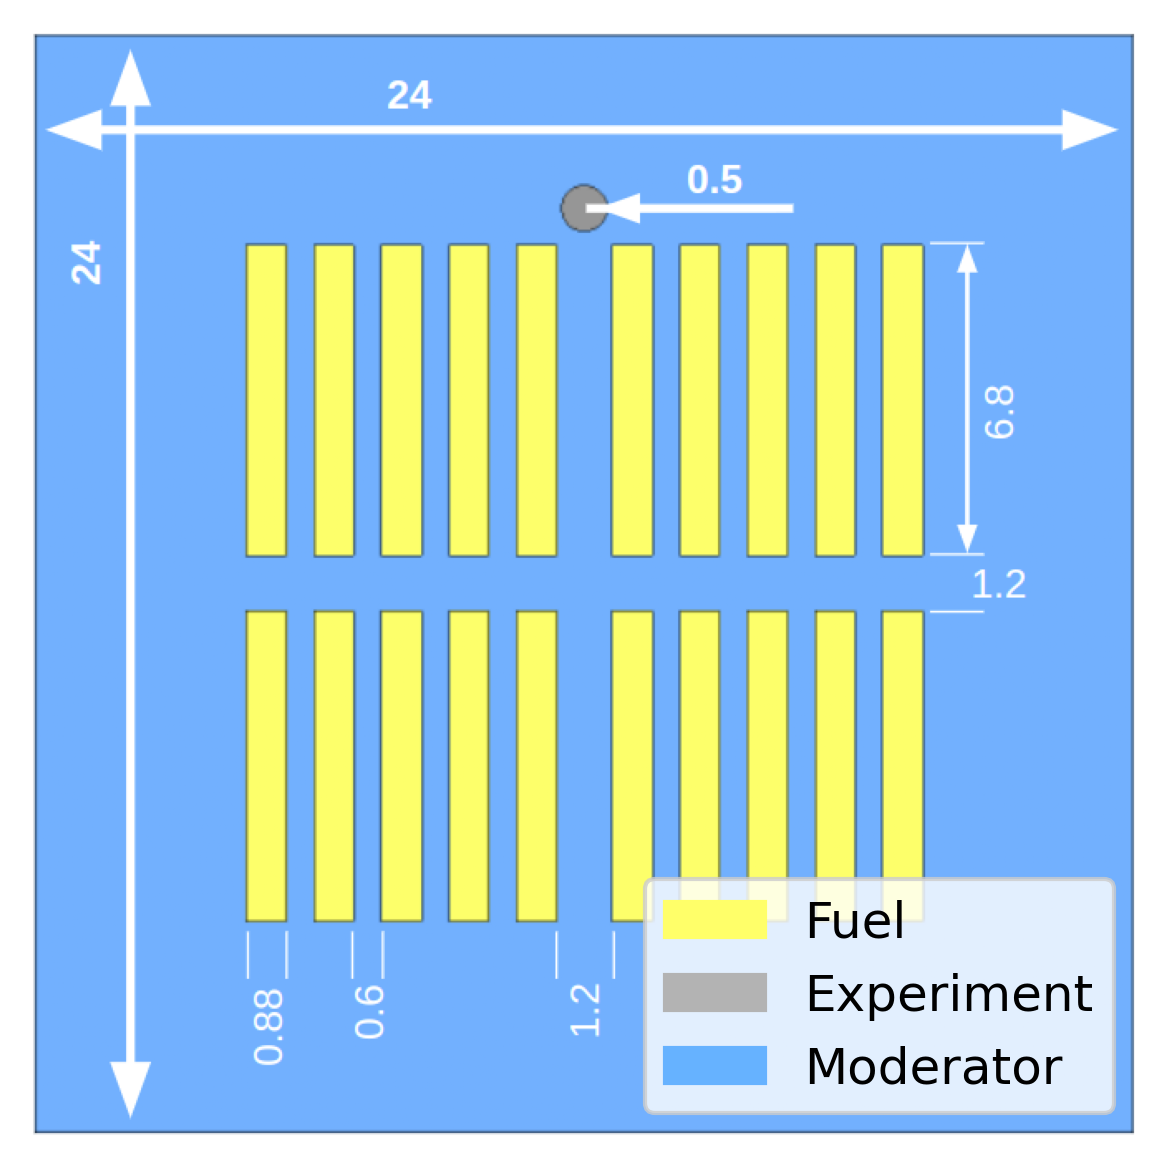
\includegraphics[width=0.50\linewidth]{figures/neutronics2-geo-legend}
    \hfill
    \caption{Geometry of the demonstration problem.}
    \label{fig:toy-geo}
\end{figure}

The experiment is irradiated for a period of 50 days with the reactor operating at a constant power of 5 MWth.
% TODO: Cross-section libraries?
After that period, the reactor shuts down, and the heat deposited in the experiment is calculated immediately after shutdown (to avoid the prompt-gamma contributions, this step is taken 1 sec after shutdown).
The reactor regions considered to contribute to the experiment heating are the fuel elements and the same experiment, while the activation of the moderator is neglected.


% This two figures could be grouped together
% total heating over time
\begin{figure}[htbp!] %or H 
    \centering
    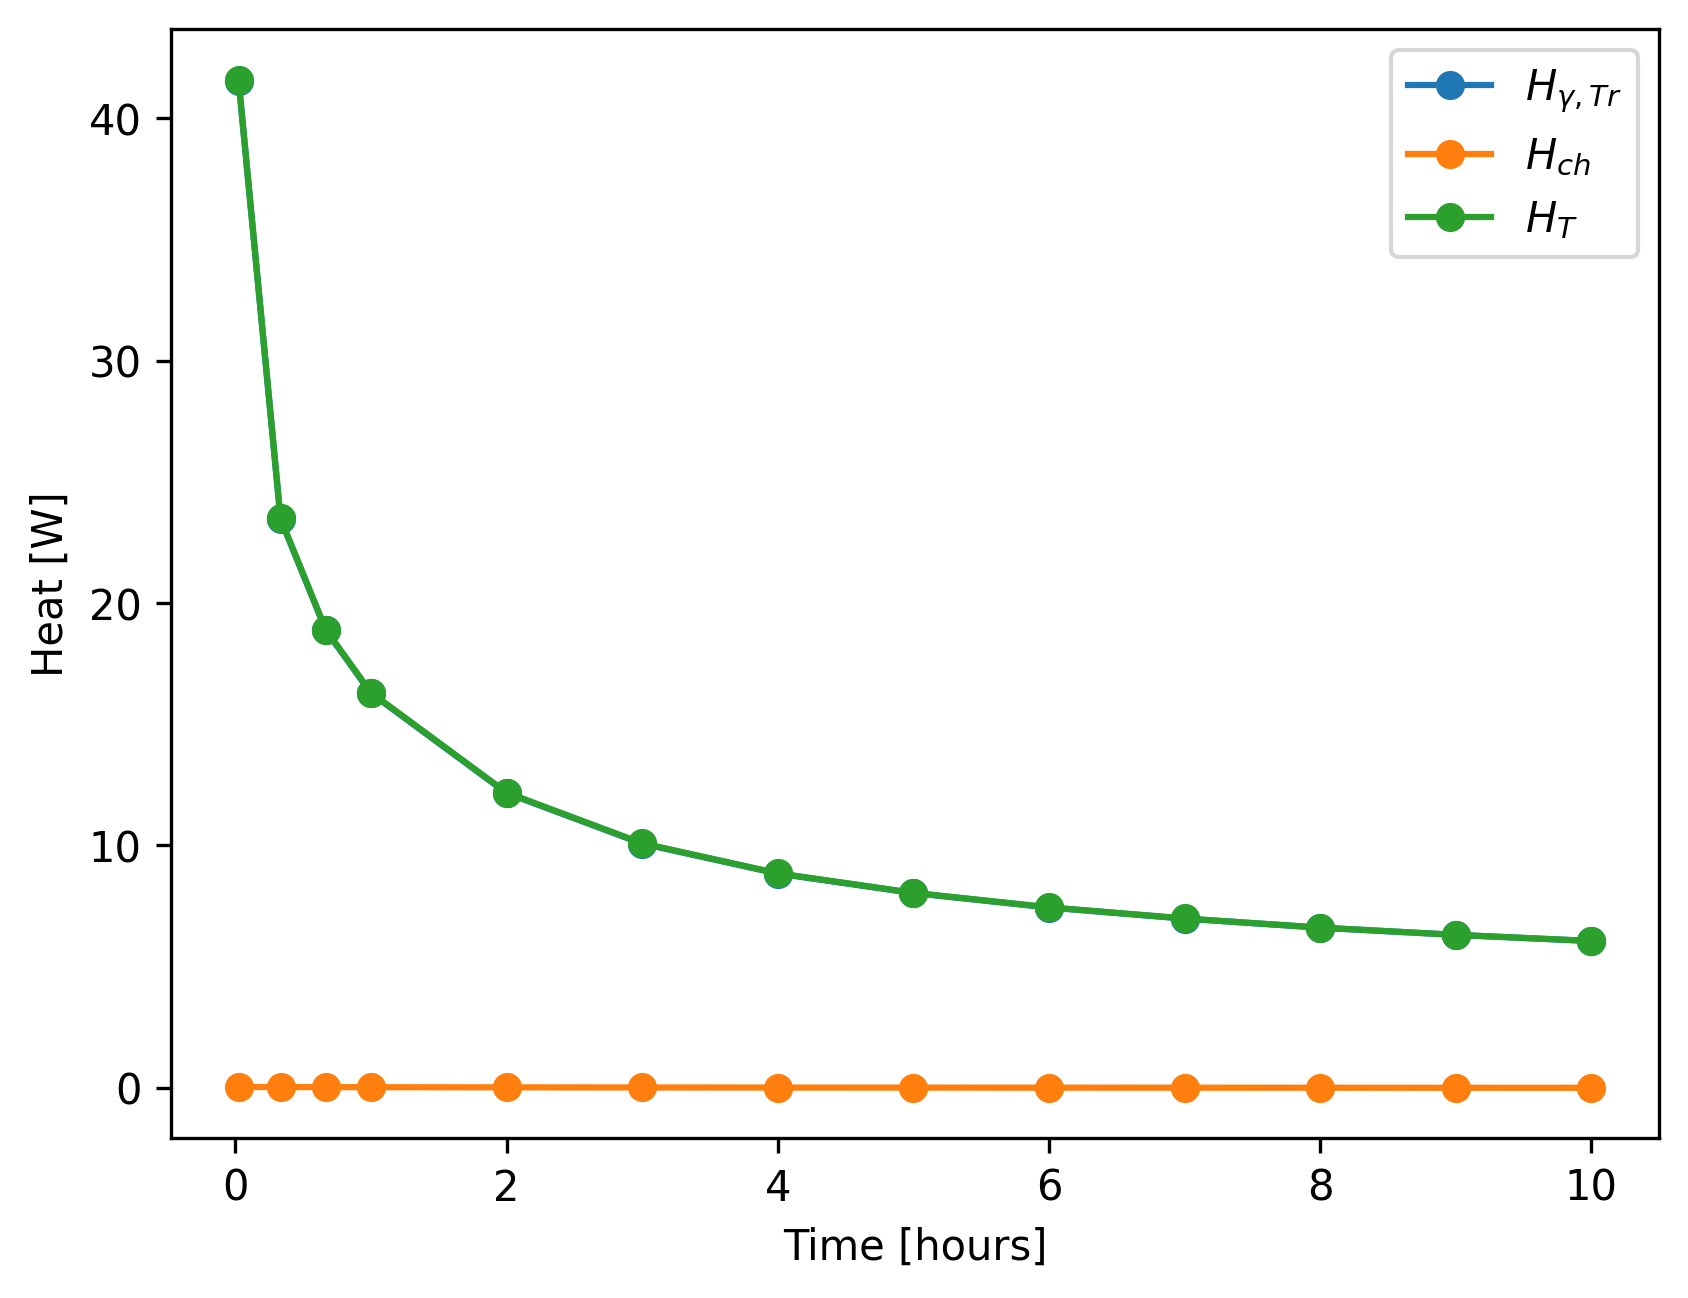
\includegraphics[width=0.55\linewidth]{figures/reference-decay-over-time}
    \hfill
    \caption{Heat production in experiment over time for the demonstration exercise.}
    \label{fig:demo-time}
\end{figure}

Figure \ref{fig:demo-time} displays the heat production over time in the experiment.
The heat produced in the experiment immediately after shutdown is 41.58 W, which is less than 0.001\% of the reactor total power.
As expected, the heat deposition has a decaying shape.
The curve has a half-life lower than 1 second, and after 4 seconds the heat production becomes smaller than 10 W.

% heat contribution by source
\begin{figure}[htbp!] %or H 
    \centering
    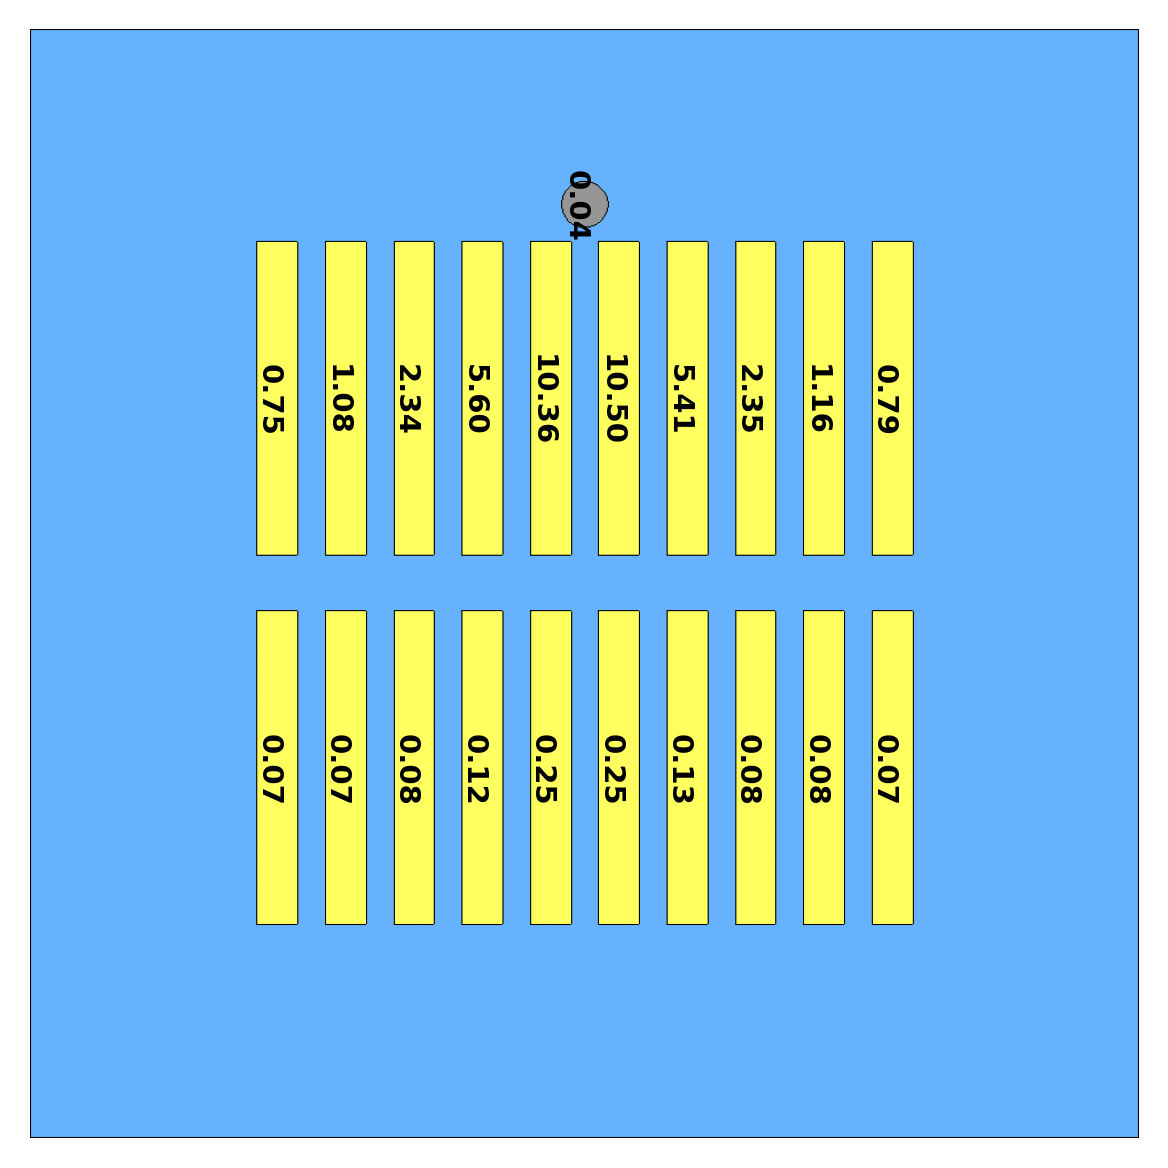
\includegraphics[width=0.70\linewidth]{figures/reference-contribs}
    \hfill
    \caption{Heat contribution by each source immediately after shutdown. Values expressed in \textit{W}.}
    \label{fig:demo-contrib}
\end{figure}

Figure \ref{fig:demo-contrib} shows the heat contribution by source.
The fuel elements contribute to the experiment heating via the deposition of the gamma radiation that originates in them.
The largest contribution to the heat deposition is originated in the closest fuel elements to the experiment.
The experiment self-heating is a combination of the energy deposition of the charged particles and gamma radiation originating in the same experiment.
The experiment material is not considerably activated during the irradiation period, and the self-heating contribution is deemed negligible.


\subsection{ATR experiment}
\label{sec:atrexp}

% % TO INCLUDE SOMEWHERE:
% % tomberlin_advanced_2002
% Two general types of experiments:
% A pressurized water loop (PWL) type of experiment that circulates water at typical pressure and temperature of an LWR.
% Capsule experiments irradiated inside the reactor pressure vessel, which rely on the reactor primary coolant for heat dissipation.

% Capsules may be any length up to 122 cm.

% % noauthor_i-loop_2019
% (1) pressurized water loop in-pile tube (IPT) experiment assemblies,
% (2) drop-in capsule irradiation assemblies
% (3) instrumented lead capsule assemblies.

% The first experiment type is positioned in an IPT that isolates the experiment from the reactor coolant and provides a way to control the experiment environment in terms of pressure, temperature, coolant flow, and chemistry.
% The second is a drop-in capsule fixed in a core or a capsule irradiation tank position and cooled by reactor primary coolant.
% The third type is a lead capsule experiment fixed in a core or a capsule irradiation tank position with instrumentation lines that exit the experiment and the reactor vessel and are connected to a control system for monitoring and controlling operating parameters.

% Intro - Why do we care about this.
The calculation scheme presented in this work is reactor-agnostic, meaning that it can be tailored to any research reactor.
Section \ref{sec:demo} calculated the delayed heating in a simple configuration, which eases the visualization of the calculation scheme.
This section demonstrates the calculation scheme for a full-scale research reactor, the \gls*{ATR}.

% ATR: Intro
The \gls*{ATR} is a 250-MWth high flux test reactor located at the Reactor Technology Complex of the \gls*{INL}.
The ATR was designed to provide an irradiation test environment for conducting a variety of experiments, to study the effects of radiation on reactor structural and fuel materials, and to produce medical and industrial isotopes \cite{ICSBEP, tomberlin_advanced_2002}.

% ATR: reactor description
The ATR core contains 40 fuel elements arranged in a serpentine annulus between and around nine flux traps, as shown in Figure \ref{fig:atr}.
Each fuel element consists of 19 parallel, curved, aluminum-clad fuel plates forming a 45-degree sector of a right circular cylinder.
The fuel arrangement gives the reactor core a clover-leaf configuration, which allows the \gls*{ATR} to be operated at different power levels in the corner lobes, allowing for independent testing conditions within the same operating cycle.
Within each fuel plate, the fuel meat consists of highly enriched (93 wt\%) uranium aluminide (UAl$_x$) fuel powder dispersed in aluminum.
Plates 1 through 4 and 16 through 19 contain natural boron carbide (B$_4$C) powder as a burnable poison.

% ATR figure of the model
\begin{figure}[htbp!] %or H 
    \centering
    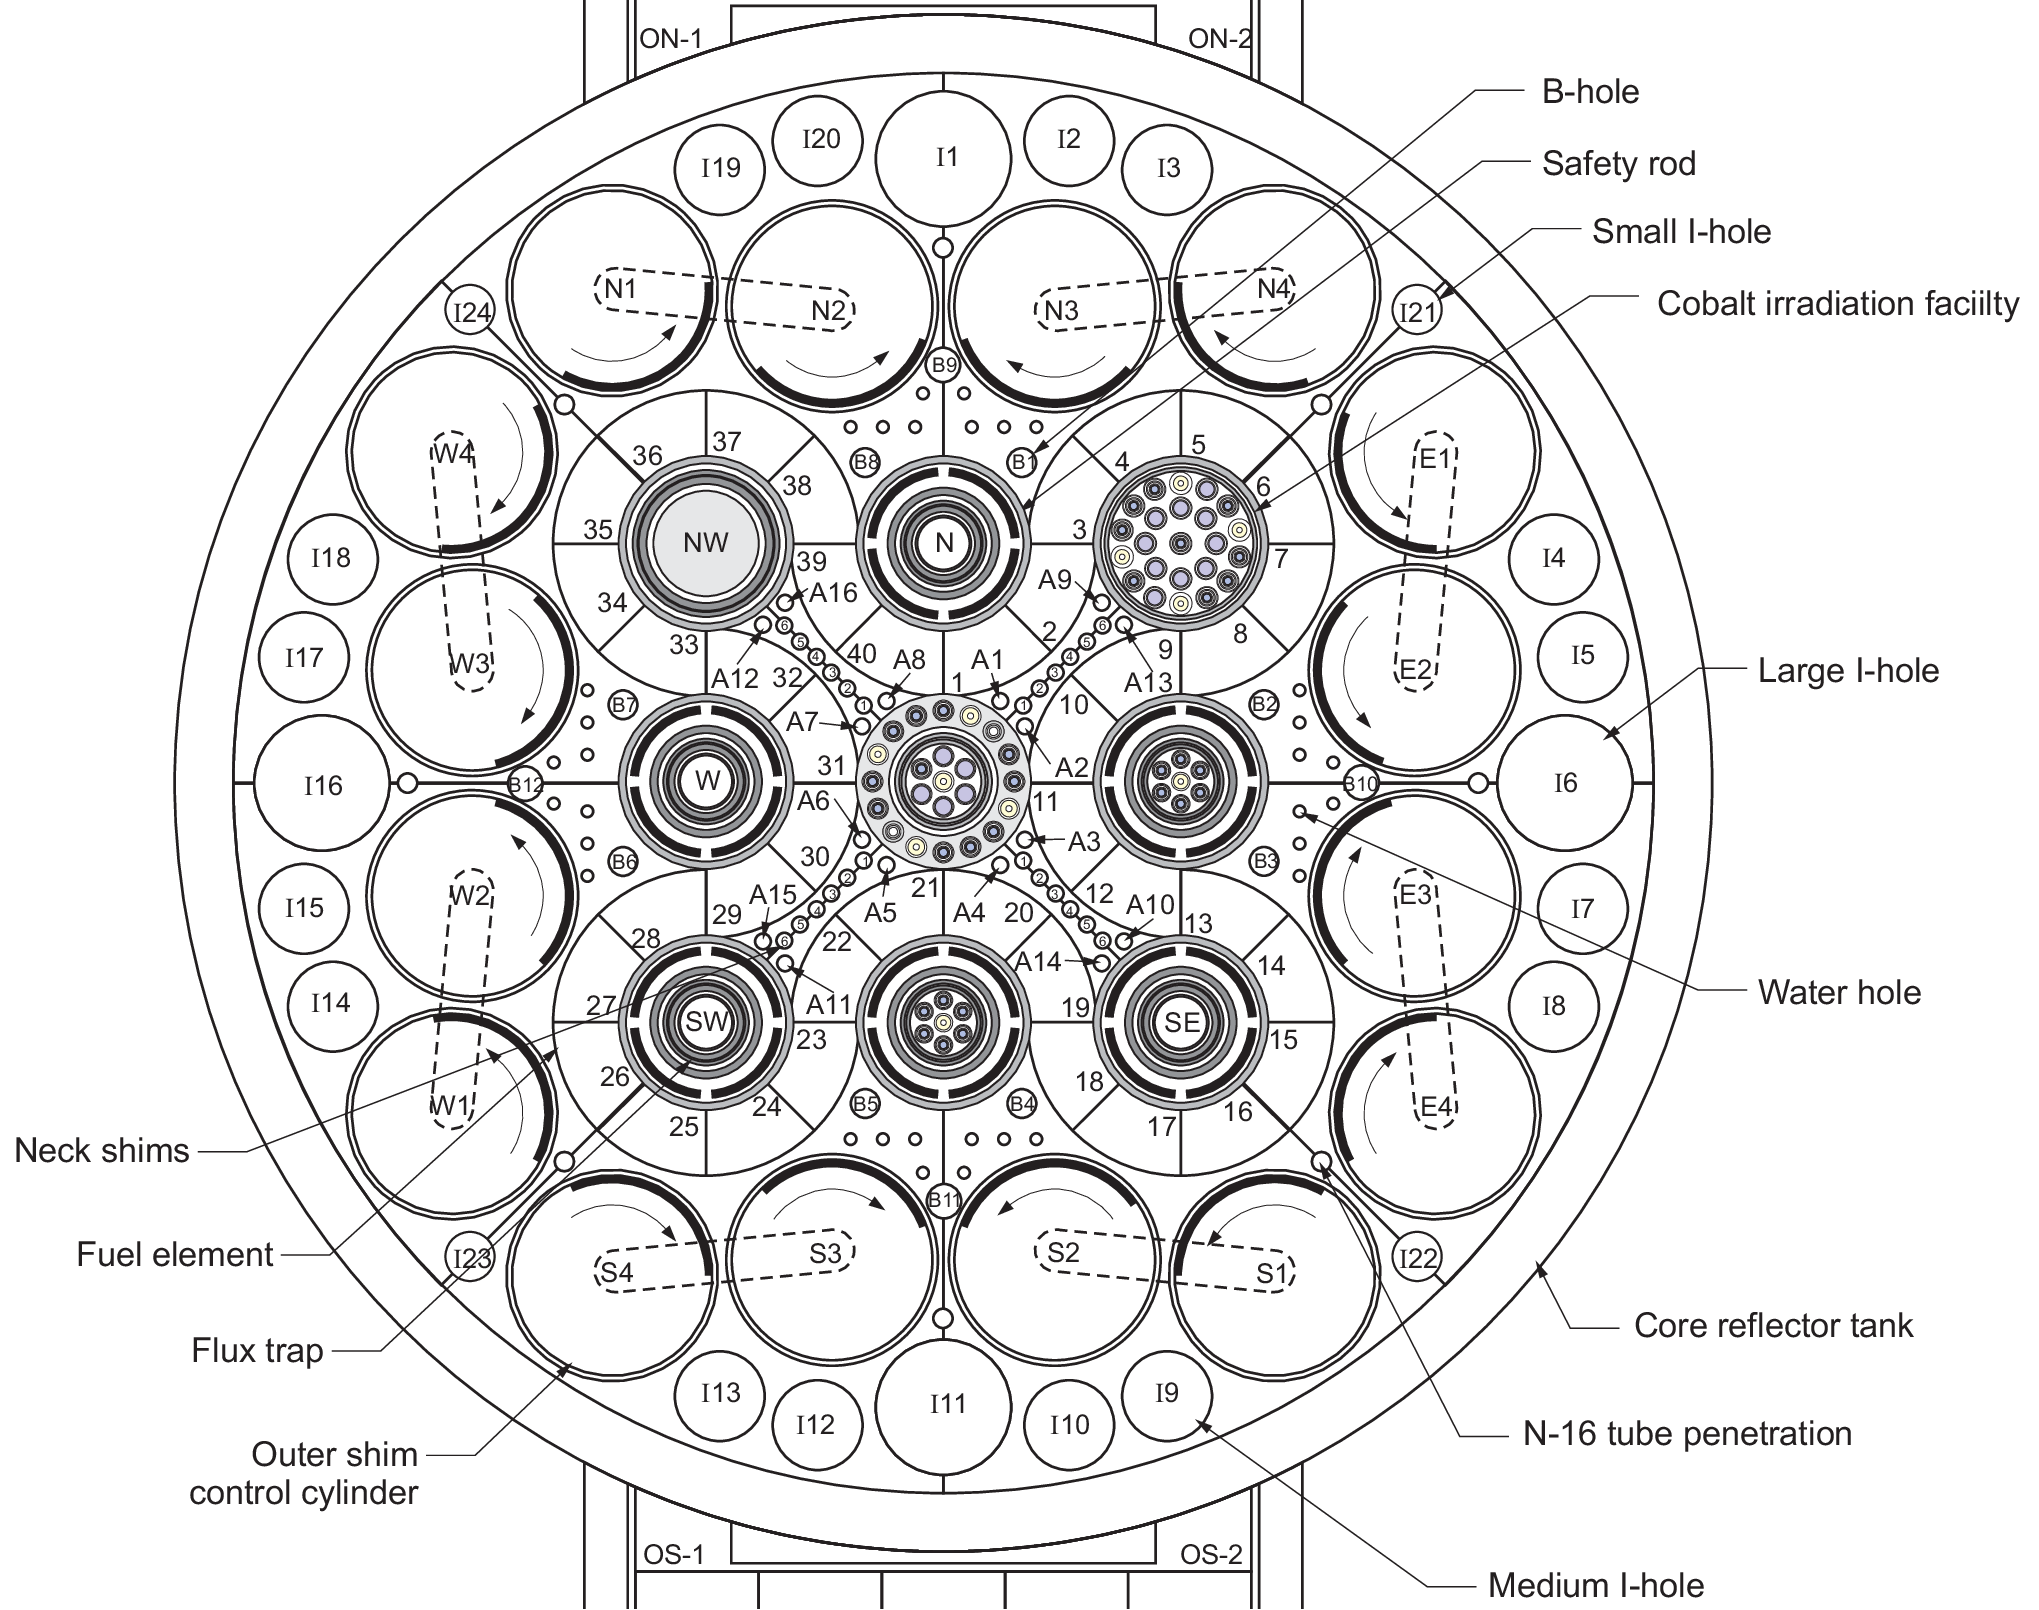
\includegraphics[width=0.85\linewidth]{figures/atr2}
    \hfill
    \caption{Top view of the ATR. Image reproduced from \cite{ICSBEP}.}
    \label{fig:atr}
\end{figure}

% Experiment positions
The reactor has 9 flux trap positions and 68 additional irradiation positions inside the reactor core reflector tank.
The center capsule facility is surrounded by the H-hole irradiation facility, which contains 10 cobalt baskets, 4 flux monitor holders, and 2 N-16 flow tubes.
The neck shim housing is the structural guide for the 24 neck shim and regulating rods, as well as 8 inner and 8 outer A-holes.
The beryllium reflector fills the space between the fuel annulus and the core reflector tank, and it hosts the outer shim control cylinders (OSCC), irradiation holes, and water holes.
The irradiation holes include a total of 8 small B-holes, 4 large B-holes, 4 small I-holes, 16 medium I-holes, 4 large I-holes, and 4 round and 4 square N-16 monitor holes.

% Describe model
This work uses an MCNP model representing the ATR critical experiment evaluation designated as Cycle 103A-2 that was performed in 1994.
This critical evaluation was part of a nuclear re-qualification program that followed the core internals change-out.
The critical configuration was defined by the following parameters: 40 fresh fuel elements, OSCC set to 51.8 degrees, 22 shim rods fully inserted, 2 regulating rods fully withdrawn, and 6 safety rods fully withdrawn.

The ATR critical evaluation was published by the OECD NEA Nuclear Science Committee in the September 2005 Edition of the International Handbook of Evaluated Criticality Safety Benchmark Experiments (ICSBEP Handbook) \cite{ICSBEP}.
% ATR-FUND-RESR-001 was approved by the IRPhEP in October of 2008 and is published in the International Handbook of Evaluated Reactor Physics Benchmark Experiments under its ICSBEP Identifier, HEU-MET-THERM-022.
% % The report is published in the original ICSBEP format and contains only evaluation of the critical state measurement.
The original benchmark model uses the evaluated continuous energy ENDF/B-V cross-section data for 27 $^{\circ}$C.
% TODO/MAYBE: make sure that I am using this cross-section library
This work uses the ENDF/B-VIII.0 cross-section library for the isotopes included in it.
The remaining isotopes use the cross-section data of the original model.
% The benchmark model 
The model uses 10$^4$ histories per generation with 250 and 3750 inactive and active cycles.
This work considers the reactor composition at the \gls*{BOC} based on the available ATR model.

% Problem definition
This demonstration exercise focuses on the delayed heating of the A1 experiment position.
The A1 experiment position is an inner A-hole, and it is hosted by the neck shim housing.
The diameter of the hole is 0.625 in.
This exercise considers an experiment sample made of aluminum.

% POWER
Although the ATR maximum power rating is 250 MWth, most contemporary experiments do not require such a level, and the reactor operates at a much lower power.
This work considers for the calculations a total operating power of 110 MWth that is equally distributed among the 5 lobes.
% Irradiation time
The irradiation time is 30 days, and the decay is recorded in seven non-uniformly distributed steps up to 12 hours after shutdown.
% This work considers the reactor composition at the \gls*{BOC} based on the available ATR model.
% However, nuclear heating tends to increase throughout the core depletion \cite{ilas_impact_2013}.
% A more conservative approach would then use the \gls*{MOC} or \gls*{EOC} configurations.

% Contributing cells
As the experiment position is in the core region between the fuel assemblies, the calculations assume that the fission products generate a much higher gamma source intensity than the activation products in the neighboring cells.
Hence, the contribution of the reactor components surrounding the experiment is neglected.
The only considered contributors to the heating are all the fuel plates and the experiment itself.


% ATR results
\subsection{ATR results}

% CHANGES IN MCNP INPUT
To accommodate the MOAA calculations, the MCNP input file underwent the following modifications.
The ATR model defines 19 different material compositions that all fuel elements share for their 19 different fuel plates.
The material definitions of each fuel plate were duplicated for each fuel element to allow for their independent definition.
Additionally, the volume of each fuel plate was calculated and added into the MCNP input file.

Figure \ref{fig:atr-time} presents the experiment heat production over time.
$H_{\gamma,Tr}$ was calculated for 41 independent photon-transport simulations, wherein each simulation accounts for the contribution to delayed gamma heating of each fuel assembly and the experiment itself.

The gamma heating immediately after shutdown was 849.2 W, and the heating due to charged particles was 56.32 W, which equals to 6.6\% of the total heating in the experiment.
The self-gamma heating was 5.8 W, which is equal to 0.73\% of the total delayed gamma contribution and 0.68\% of the total heating.
These results show that the self-heating in aluminum is very low and validate the initial simplification of neglecting the surrounding structure contributions given that both the experiment and the structures are made of aluminum.

Additionally, the heating due to charged particles decays much faster than the gamma heating and becomes negligible one hour after shutdown.
The gamma heating decays to 100 W at approximately six hours after shutdown.

\begin{figure}[htbp!] %or H 
    \centering
    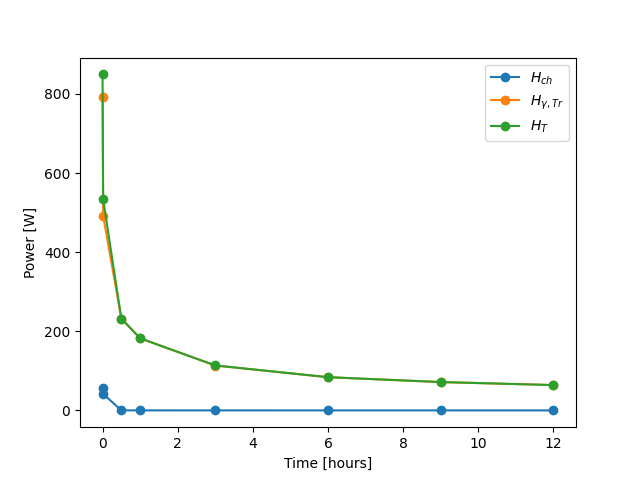
\includegraphics[width=0.65\linewidth]{figures/atr-decay-heat-time}
    \hfill
    \caption{Shutdown heating rate over time in the ATR A1 experiment position for an aluminum sample.}
    \label{fig:atr-time}
\end{figure}

Figure \ref{fig:atr-contrib} shows the contribution to the total heat in percentage by each fuel assembly and the experiment immediately after shutdown.
The largest contributions to the heating in the sample come from the fuel assemblies 1, 10, 40, 2, 11, 9 with contributions of more than 3\%.
These assemblies are the closest in distance to the experiment position.
Additionally, the sample produced a self-heating of 7.3\%, from which 6.6\% came from the charged particles, and 0.7\% from the gamma particles.
% This confirms the assumption that the gamma heating from the fission products is considerably larger than the gamma heating from activation products in the vicinity of the fuel assemblies.

% Maybe talk about the following:
% The neck shim housing has an elongated shape.
% So, several of the gammas originated here will not be deposited in the experiment position but in the fuel elements.
% Additionally, our method considers that the gamma are originated uniformly across the cell geometry.
% Which in this case a mesh based approach may be more accurate.

\begin{figure}[htbp!] %or H 
    \centering
    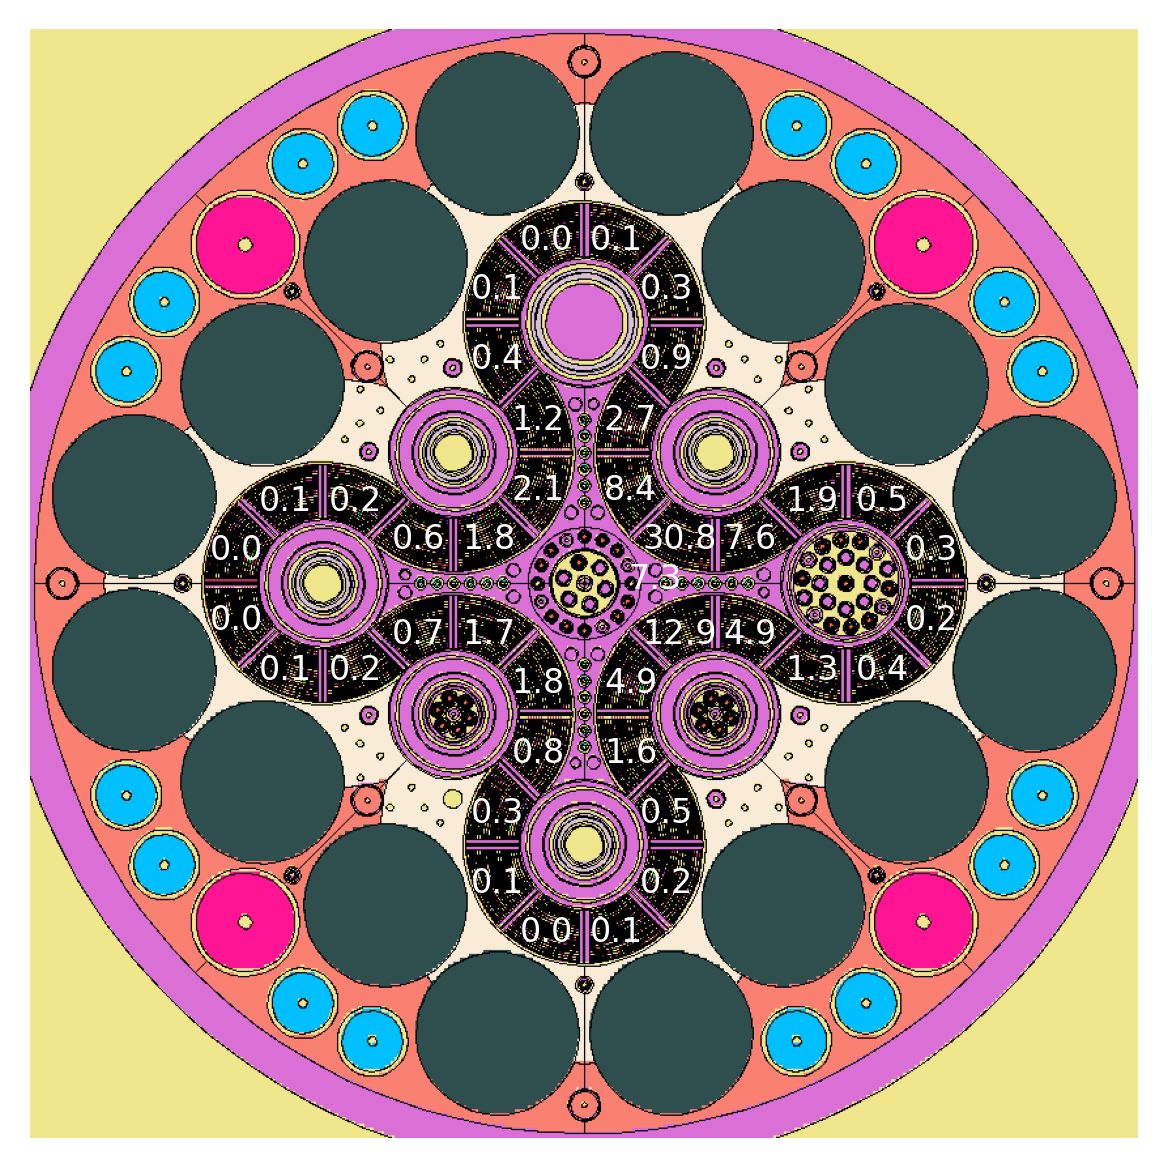
\includegraphics[width=0.90\linewidth]{figures/atr-contributions}
    \hfill
    \caption{Contribution by each source to the A1 experiment heat rate immediately after reactor shutdown, with the values expressed in (\%). The Figure is based on the MCNP model geometry, which is rotated 45$^{\circ}$ clockwise with respect to Figure \ref{fig:atr}.}
    \label{fig:atr-contrib}
\end{figure}


\subsection{RA-6 structures}

% Intro
The RA-6 is a 3-MWth open pool research reactor located at the Bariloche Atomic Center (CAB), a research and development center of the Argentine National Atomic Energy Commission (CNEA) \cite{ICSBEP}.
It was originally conceived as a teaching tool to support student training at the Balseiro Institute before its uses became diversified.
Current applications include neutron activation analysis, neutron radiography, and \gls*{BNCT}, among others.

% The reactor
The reactor core is composed of a fuel element arrangement, as shown in Figure \ref{fig:ra6-1}, that rests on a support grid inside a 2.4-m-diameter, 10.4-m-high stainless-steel tank.
The tank is filled with demineralized light water, which acts as a coolant, moderator, and reflector.
The fuel elements are Material Test Reactor (MTR) type, composed of rectangular fuel plates with aluminum side plates.
The fuel meat consists of 19.7\% enriched uranium silicide (U$_3$Si$_2$) dispersed in an aluminum matrix.
There are two types of fuel elements: Normal Fuel Elements (NFEs) and Control Fuel Elements (CFEs).
While an NFE is composed of 17 internal and two external fuel plates, a CFE is composed of 14 internal and 4 control guide plates.

% Support grid
The bottom plane of the core assembly rests 8.9-meters-deep on the support grid, which is a 20 cm-thick slab of 99.5\% pure aluminum.
Primary and secondary cylindrical holes allow the cooling of the internal and external fuel plates, respectively.
The primary holes have a diameter of 6.179 cm and are arranged in a rectangular 8x10 array with 7.7-cm pitch in the x-direction and 8.1-cm pitch in the y-direction.
The secondary holes have a diameter of 2.225 cm and are centered between the primary holes.

% BNCT filter
On a side of the fuel element arrangement, there is a neutron filter that works as a source for \gls*{BNCT}, as shown in Figure \ref{fig:ra6-2}.
The neutron filter for the \gls*{BNCT} facility is an 87.6-cm-long, 77.1-cm-wide, 82.35-cm-high aluminum container.
The filter is filled along the 87.6-cm dimension with the following materials: 17 cm of aluminum bricks, a 0.15-cm-thick cadmium sheet, 10 cm of aluminum, a 0.15-cm-thick cadmium sheet, and the rest is filled with alumina bricks.

\begin{figure}[htbp!] %or H 
    \centering
    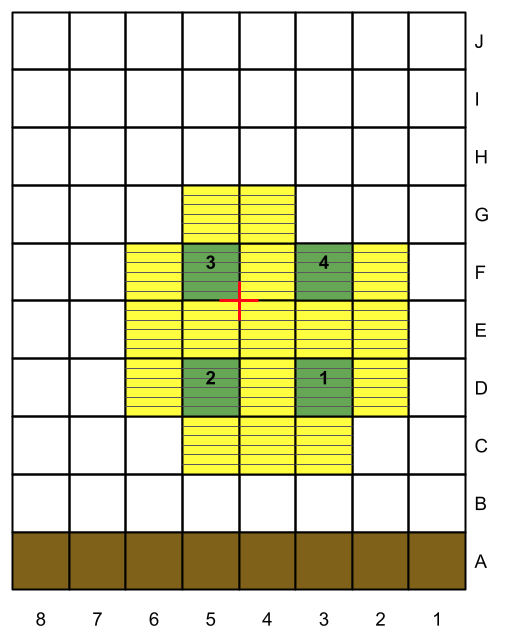
\includegraphics[width=0.50\linewidth]{figures/ra6-core2}
    \hfill
    \caption{Top view of the RA-6 critical configuration. NFEs in yellow, CFEs in green, and BNCT filter in brown. Red cross denotes the center of the reactor pool. Image reproduced from \cite{ICSBEP}.}
    \label{fig:ra6-1}
\end{figure}

\begin{figure}[htbp!] %or H 
    \centering
    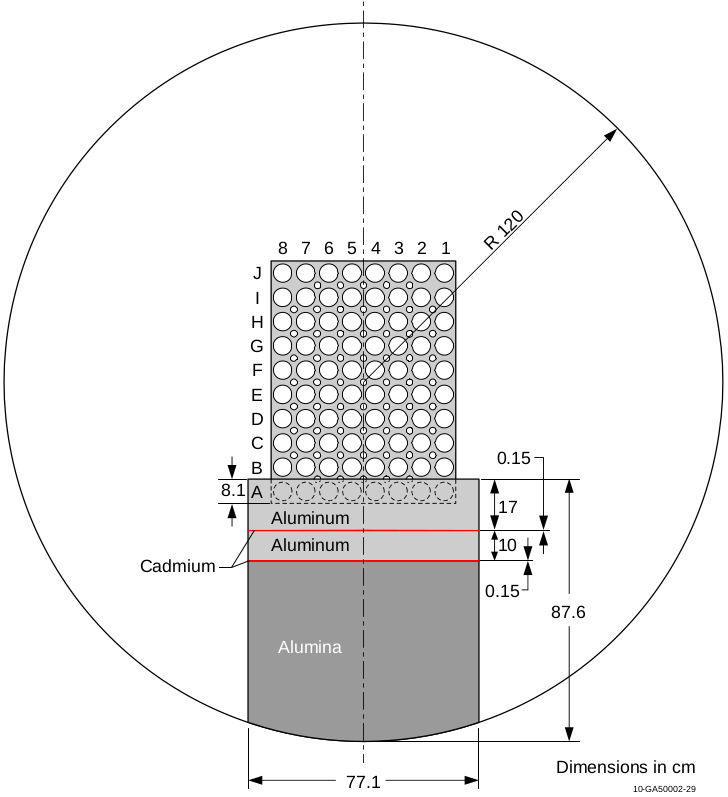
\includegraphics[width=0.65\linewidth]{figures/bnct}
    \hfill
    \caption{Top view of the RA-6 support grid and BNCT filter. Image reproduced from \cite{ICSBEP}.}
    \label{fig:ra6-2}
\end{figure}

% The model
The RA-6 reactor operated for 20 years with spent \gls*{HEU} fuel from a higher power reactor and was converted to \gls*{LEU} fuel in 2008.
The RA-6 critical experiment reported in this evaluation corresponds to the 2008 configuration utilized in the startup program.
% RA6-FUND-RESR-001 
This critical evaluation was published by the OECD NEA Nuclear Science Committee in the September 2010 Edition of the ICSBEP Handbook.
% RA6-FUND-RESR-001 was first published by the IRPhEP in the March 2013 Edition of the International Handbook of Evaluated Reactor Physics Benchmark Experiments under its ICSBEP Indentifier, IEU-COMP-THERM-014.
% The report contains only an evaluation of the critical state measurement.
This work considers the reactor composition at the \gls*{BOC} based on the available RA-6 model and uses the evaluated continuous energy ENDF66 cross-section data for 27 $^{\circ}$C, which is defined in the original benchmark model.
% % TODO/MAYBE: make sure that I am using this cross-section library
% This work uses the ENDF/B-VII.1 cross-section library for the isotopes included in it.
% The remaining isotopes use the original model cross-section data.
% The benchmark model 
The simulation uses 10$^4$ histories per generation with 50 and 4000 inactive and active cycles.

% The calculations
Although not shown in the MCNP model, the reactor core has several surrounding components, such as primary pipes, the stainless-steel tank, and neutron beam extraction tubes.
The analysis of delayed heating in these components could be worthwhile but was omitted as the MCNP model excluded them.
Hence, this work calculates the delayed heating on the most important structural components in the model, i.e., the support grid and the BNCT filter.

% POWER
The RA-6 was originally designed to operate at 1 MWth and the 2008 startup program included a reactor power upgrade to 3 MWth.
Although the RA-6 maximum power rating is 3 MWth, it normally operates at a lower power.
This work considers operating powers of 1 and 3 MWth and compared their respective results.
% Irradiation time
In this work, the rector operated for 1 year and the depletion was calculated in four 3-month steps.
% Contributing cells
The considered contributors to the heating are the fuel plates, the support grid, and the BNCT filter.


\subsection{RA-6 results}

% CHANGES IN MCNP INPUT
To accommodate the MOAA calculations, the MCNP input file underwent the following modifications.
First, even though the RA-6 model distinguishes between five different types of fuel plates: internal plates in the nuclear fuel elements (NFEs), internal plates with burnable poisons in the NFEs, external plates in the NFEs, fuel plate with burnable poisons in the control fuel elements (CFEs), and fuel plate without burnable poisons in the CFEs, the original MCNP input file defines all of them with the same material definition.
Additionally, several layers of the BNCT filter and the support grid are made of pure aluminum, and the original MCNP input file defines the material aluminum only once.
The BNCT filter also uses two cadmium layers that share the same material definition in the original MCNP input file.
All material definitions of these components were duplicated to allow for their independent definition.
Second, the original MCNP input file defines the four CFEs using nested structures with independent cells, but as their definition is identical, a minimal universe renumbering allowed for their simultaneous modeling in MOAA.
Third, the volume of each fuel plate type, the volume of the different BNCT filter layers, and the volume of the support grid were calculated and added into the MCNP input file.

Figure \ref{fig:ra6-3} shows the delayed heating in the support grid and the different BNCT filter layers for operating powers of 1 and 3 MWth, and Table \ref{tab:ra6-res} shows the deposited heat density in the different structures.
The highest deposited heat occurs in the first BNCT layer, while the highest deposited heat density occurs in the second BNCT layer, which is the first cadmium layer in the filter.
For the first, third, and fifth layers of the BNCT filter, the deposited heat density decreases due to an increase in the spatial distance from the core.
However, the fifth layer has a larger deposited heat than the third layer due to its considerably larger volume.
The deposited heat in the cadmium sheets is considerably smaller than for the rest of the BNCT layers due to their smaller volume.
Table \ref{tab:ra6-res} also shows the comparison between the results for 1 and 3 MWth.
An increase in operation power of 200\% translated into an increase in delayed heating of between 160-190\% for the reactor structures.

\begin{figure}[htbp!] %or H 
    \centering
    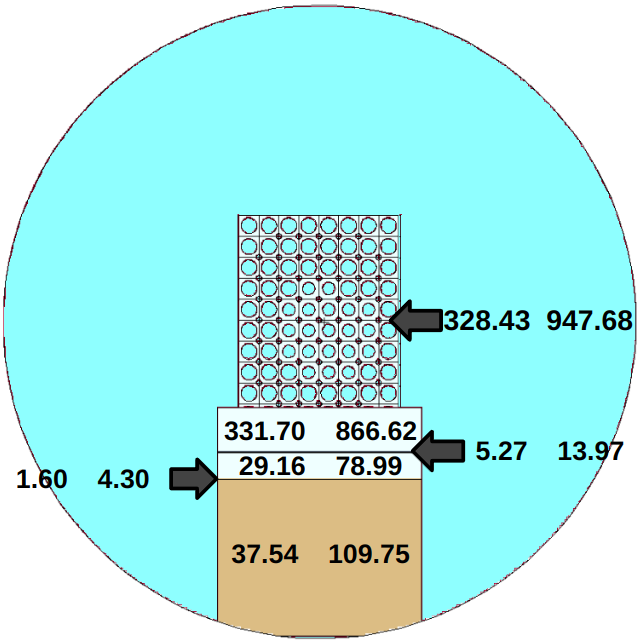
\includegraphics[width=0.75\linewidth]{figures/results_b}
    \hfill
    \caption{Delayed heating in the RA-6 reactor structures. Values expressed in $W$. Left: values corresponding to 1 MWth. Right: values corresponding to 3 MWth.}
    \label{fig:ra6-3}
\end{figure}

\begin{table}[htbp!]
  \centering
  \caption{Main results for delayed heating in the RA-6 reactor structures for operating powers of 1 and 3 MWth.}
  \label{tab:ra6-res}
  \begin{tabular}{cccc}
    \toprule
                    % & $H_{T, 1MW}/V [W/m^3]$  & $H_{T, 3MW}/V [W/m^3]$  & $ \frac{H_{T, 3MW}}{H_{T, 1MW}} - 1$  \\
                    & $H_{T, 1MW}/V [W/m^3]$  & $H_{T, 3MW}/V [W/m^3]$  & Rel. Diff. [\%]  \\
    \midrule
    Support grid    &  3291.14                &  9496.55                &  189 \%   \\
    BNCT 1st layer  &  3073.12                &  8029.02                &  161 \%   \\
    BNCT 2nd layer  &  5533.52                & 14668.54                &  165 \%   \\
    BNCT 3rd layer  &   459.27                &  1244.10                &  171 \%   \\
    BNCT 4th layer  &  1680.01                &  4515.01                &  169 \%   \\
    BNCT 5th layer  &   102.13                &  298.57                 &  192 \%   \\
    \bottomrule
  \end{tabular}
\end{table}


\section{Conclusions}

% Use conclusions from prelim and 8 and make specific to this thesis
% FROM 8-
% Intro
Safety analyses in research reactors require the estimation of heat deposited in experiments and reactor structures after reactor shutdown.
These analyses establish the heat-source term of those components, and the subsequent thermal-hydraulics calculations determine if an accident could jeopardize their integrity.
Additionally, detailed calculations help guide the optimization process of the design of irradiation targets.

In general, existing research reactor safety analyses have a strong focus on the reactor core and assume that the energy released after shutdown is deposited locally in the region of interest.
Moreover, many software packages rely on the same assumption, which may be inadequate in some cases.
On the other hand, an accurate assessment of the deposited energy across the reactor geometry allows for better determination of the heat removal requirements and ensures an effective cool down.
Instead of assuming locally deposited heat, this work utilizes detailed methods to target the specific reactor regions.

% Background
Chapter \ref{ch:lit} discussed various delayed heating calculation methods, and several publications relying on them.
The fact that the formal 3-step process accounts for the activation product decay and the time evolution after shutdown makes it better suited for this thesis than other methods.
Therefore, this chapter introduced a delayed heating calculation workflow based on the formal 3-step process that relies on MOAA.

% MOAA
MOAA is a Python package that couples MCNP and ORIGEN to streamline the calculation of the experiment source terms for experimental reactors.
This chapter described MOAA's workflow and the delayed heating calculation workflow and several practical aspects of the simulations.
The delayed heating calculation relies on MOAA for conducting the first two steps of the process, while the third step is conducted by multiple MCNP photon transport simulations.

% Results
Finally, this chapter demonstrated the delayed heating calculation capabilities by presenting four exercises.
The first exercise consisted of a code-to-code comparison between the workflow presented here and the Serpent Monte Carlo tool.
The purpose of this exercise was to understand the foundation of the method by comparing the results with Serpent.
The second exercise demonstrated the calculation workflow for a simple case geometry.
This exercise allows to better visualize the method and current capabilities.
The third and fourth exercises focus on full-size reactor exercises.
These exercises include the delayed heating in an ATR experiment and the RA-6 structures.
For the ATR experiment, the results showed the time evolution of the delayed heating up to 12 hours after shutdown, as well as the contribution to the heating from the different sources in the reactor.
For the RA-6 structures, the results displayed the delayed heating in several of the structural components and the comparison of the heating values for different power levels.

% Conclusions
As discussed in the results section, the calculation workflow can accommodate almost any MCNP input file, with some minimal modifications.
This workflow streamlines the calculation of delayed heating in research reactor experiments necessary for the development of experiment safety analysis.
Overall, this chapter presented delayed heating capabilities that rely on MOAA and that can be applied to any reactor.
